%% LaTeX_Thesis_Template.tex
% An unofficial LaTeX template for Cranfield theses.
% 2017/08/14 Daniel Auger's unofficial Cranfield thesis .sty file
% 2023/05/31 Updated by Shaun Forth (SAF) for logo inclusion
% 2023/06/08 SAF removed capitalisation on title pages on advice of Amy 
% Greenaway and Alison Waters. Added Daniel Auger's headers with 
% chapter and section names.
% 2023/06/08 SAF simplified logo inclusion

%%
% This document is an example of the use of the unofficial "cranfieldthesis" 
% LaTeX style file.  I hope it's useful, and a good likeness of the Word template.

\documentclass[12pt,oneside]{book} % for one-sided printing
%\documentclass[12pt,twoside]{book} % for two-sided printing

% Use the custom "cranfieldthesis" LaTeX style file. 
\usepackage{cranfieldthesis}
\usepackage{lscape} % for landscape pages
\usepackage{amsmath}
\usepackage{enumitem}
\usepackage{changepage}
\usepackage{pdfpages}
\usepackage{blindtext}% Just used so we can generate some example text
\usepackage{algorithm}
\usepackage{algpseudocode}
\usepackage{amssymb}
\usepackage{mathtools}
\usepackage[export]{adjustbox}
\usepackage{lipsum}
\usepackage{booktabs}  % For better quality tables
\usepackage{siunitx}
\usepackage{float}
\usepackage{longtable} % Pour les tableaux sur plusieurs pages
\usepackage{tabularx}  % for the X column type
\usepackage{listings}
\usepackage{xcolor}
\usepackage{caption}
\usepackage{xfrac}
\usepackage{indentfirst}
\usepackage{subcaption}
\usepackage{graphicx}
\usepackage{geometry}
\usepackage{titlesec}
\usepackage{multirow}
\usepackage{adjustbox} % To adjust the table size
\geometry{a4paper, margin=1in}
\hypersetup{
    colorlinks,
    linkcolor={blue!50!blue},
    citecolor={blue!50!blue},
    urlcolor={blue!80!blue}
}

% By default, LaTeX uses a serif font - these are traditionally thought to be
% easier to read.   If you'd prefer sans-serif, please uncomment the 
% following line.
% \renewcommand{\familydefault}{\sfdefault}

% Example parameters for a typical taught MSc course
\title{Future Position Prediction for Pressure Refuelling Port
    of Commercial Aircraft}
\author{Alexis Balayre}
\date{May 2024}
\school{\SATM}
\course{Computational and Software Techniques in Engineering}
\degree{MSc}
\academicyear{2023--2024}
\setCUPartnerLogo{logo-airbus.png}
\supervisors{Dr Boyu Kuang and Dr Stuart Barnes}
\copyrightyear{2024}

% References
% Cranfield Numbered Style
\usepackage[numbers]{natbib} % for nice referencing
\makeatletter % Reference list option change to number and period
\renewcommand\@biblabel[1]{#1.} % from [1] to 1
\makeatother %

\begin{document}

%% Front matter
%
% This is where we do the title page, etc.
%

\frontmatter

% Standard-Form Title Pages
\maketitle

% Abstract and Keywords
\begin{abstract}
    Replace with your abstract text of not more than 300 words.
\end{abstract}

\begin{keywords}
    Replace with at least 6, semicolon seperated keywords (not contained within the thesis title) – this makes the thesis searchable.
\end{keywords}

% Acknowledgements
\chapter{Acknowledgements}
 %The author would like to thank \dots

 % Use single spacing for Table of Contents, List of Figures, etc
 {
  \clearpage

  % Table of Contents
  \singlespacing{
      \tableofcontents
  }
  \clearpage

  % List of Figures
  {%
      \let\oldnumberline\numberline%
      \renewcommand{\numberline}{\figurename~\oldnumberline}%
      \listoffigures%
  }

  \clearpage
  % List of Tables
  {%
      \let\oldnumberline\numberline%
      \renewcommand{\numberline}{\tablename~\oldnumberline}%
      \listoftables%
  }
 }

% The list of abbreviations can't be automatically generated so you need to populate it yourself
\begin{listofabbreviations}
    \abbrev{ML}{Machine Learning}
    \abbrev{DL}{Deep Learning}
    \abbrev{AI}{Artificial Intelligence}
    \abbrev{CNN}{Convolutional Neural Network}
    \abbrev{RNN}{Recurrent Neural Network}
    \abbrev{LSTM}{Long Short-Term Memory}
    \abbrev{GRU}{Gated Recurrent Unit}
    \abbrev{EKF}{Extended Kalman Filter}
    \abbrev{AAGR}{Autonomous Aircraft Ground Refueling}
    \abbrev{AGR}{Aircraft Ground Refueling}
    \abbrev{UAV}{Unmanned Aerial Vehicle}
    \abbrev{AAR}{Autonomous Aerial Refueling}
    \abbrev{DGPS}{Differential Global Positioning System}
    \abbrev{SVM}{Support Vector Machine}
    \abbrev{HOG}{Histogram of Oriented Gradients}
    \abbrev{SOTA}{State-of-the-Art}
    \abbrev{AIS}{Automatic Identification System}
    \abbrev{GPS}{Global Positioning System}
    \abbrev{IoU}{Intersection over Union}
    \abbrev{TP}{True Positive}
    \abbrev{FP}{False Positive}
    \abbrev{FN}{False Negative}
    \abbrev{TN}{True Negative}
    \abbrev{AP}{Average Precision}
    \abbrev{AR}{Average Recall}
    \abbrev{SSD}{Single Shot Multibox Detector}
    \abbrev{YOLO}{You Only Look Once}
    \abbrev{IoT}{Internet of Things}
    \abbrev{AFRL}{Air Force Research Laboratory}
    \abbrev{AR3P}{Autonomous \& Robotic Remote Refueling Point}
    \abbrev{BIPRS}{Brightness Invariant Port Recognition System}
\end{listofabbreviations}

%% Main Matter
%
% This is where we include the main thesis content.
%
\mainmatter\pagestyle{fancy}
\fancyhead[L]{\nouppercase{\leftmark}}
\fancyhead[R]{\nouppercase{\rightmark}}

%%%%%%%%%%%%%%%%%%%%%%%%%%%%%%%%%%%%%%%%%%%%%%%%%%%%%%%%%%%%%%%%%%%%%%%%%%%%%%%%
%%%%%%%%%%%%%%%%%%%%%%%%%%%%%%%%% INTRODUCTION %%%%%%%%%%%%%%%%%%%%%%%%%%%%%%%%%
\chapter{Introduction}
\section{Background and Motivation}

Ground pressure refuelling is a standard method used to refuel commercial
aircraft safely and efficiently. This process involves using a system of
underground fuel pipelines and hydrants at aircraft parking
spots~\cite{blakey2011aviation}. When an aircraft is ready for refueling, a
hydrant dispenser vehicle connects to the hydrant pit and delivers fuel to the
aircraft through a flexible hose~\cite{sati2019aircraft} (see
Figure~\ref{fig:pressure-refuelling}). This method allows for high fuel flow
rates and significantly reduces aircraft turnaround
times~\cite{blakey2011aviation}. However, this process also presents several
challenges, particularly in terms of safety and accuracy. In the past, there
have been several incidents involving ground pressure refueling, including fuel
spills, overfills, and equipment
failures~\cite{doi:10.1080/13669877.2013.879493, CostsOfUnsafetyAviation}.
Fortunately, with the advancement of technology, many of these challenges will
be addressed, and the refueling process will become safer and more efficient. 

\begin{figure}[H]
    \centering
    \includegraphics[width=0.5\textwidth]{figures/pressure-refuelling.jpeg}
    \caption{Pressure Refuelling of a Commercial Aircraft. Photo Credit: Tom Boon/Simple Flying~\cite{ImageRefueling}}\label{fig:pressure-refuelling}
\end{figure}

The aviation industry is undergoing a significant transformation with the
development of the airport of the future, commonly known as `Smart Airport’ or,
more recently, `Airport 4.0’. The concept of Smart Airport encompasses the use
of cutting-edge information technologies, such as the Internet of Things (IoT),
Artificial Intelligence (AI), and Blockchain, to monitor, analyse, and
integrate real-time data on the airport's status. This integration aims to
achieve optimal operational efficiency and enhance the quality of service.
Taking the concept a step further, Airport 4.0 envisages an airport driven
entirely by AI, capable of making autonomous decisions thanks to self-learning
mechanisms. This advance aims to automatically predict and manage various
airport scenarios, making it easier to automate numerous processes. The result
is a substantial reduction in operating costs and error
rates~\cite{10.1007/978-981-16-5943-0_26}.

Among these, automated refuelling systems play a crucial role in ensuring
efficient and accurate refuelling of aircraft. However, one of the main
challenges of this automation process is the accurate detection of the
aircraft's refuelling port, which is relatively small and can easily be
obscured by other visual elements on or near an aircraft. For example in the
Figure~\ref{fig:challenges-detecting-ports}, the refuelling port is located on
the wing of the aircraft and can be difficult to detect due to motion blur,
occlusion, or being out of view. This challenge is further compounded by the
fact that aircraft refuelling ports can vary in size, shape, and location
depending on the aircraft type and manufacturer. Scanning the entire area of
each video frame is both time-consuming and inaccurate. It is therefore
essential to develop a more efficient and accurate method of locating the
refuelling port. 

% 4 Images
\begin{figure}[H]
    \centering
    \begin{subfigure}[b]{0.3\textwidth}
        \includegraphics[height=0.7\textwidth, width=\textwidth]{figures/image_hard_2.jpg}
        \caption{Motion Blur Example}\label{fig:motion-blur-example}
    \end{subfigure}
    \hfill
    \begin{subfigure}[b]{0.3\textwidth}
        \includegraphics[height=0.7\textwidth, width=\textwidth]{figures/image_hard_4.jpg}
        \caption{Occlusion Example}\label{fig:occlusion-example}
    \end{subfigure}
    \hfill
    \begin{subfigure}[b]{0.3\textwidth}
        \includegraphics[height=0.7\textwidth, width=\textwidth]{figures/image_hard_3.jpg}
        \caption{Out-of-View Example}\label{fig:out-of-view-example}
    \end{subfigure}
    \caption{Challenges in Detecting Aircraft Refuelling Port}\label{fig:challenges-detecting-ports}
\end{figure}

\section{Research Gap}
Despite significant advancements in autonomous aircraft ground refuelling
technologies, critical challenges remain, particularly in the accurate
detection and positioning of the refuelling port. The small size and varied
locations of refuelling ports, often obscured by visual elements like motion
blur and occlusions, complicate this task. Existing systems have made progress
using machine vision, but they are limited by inefficiencies in scanning entire
video frames and inaccuracies under different environmental conditions.
Furthermore, while current methodologies leveraging convolutional neural
networks (CNNs) and Kalman filters have improved detection accuracy, they still
struggle with real-time performance and adaptability in dynamic environments.
The robustness of these systems in varied lighting conditions and their
capability to handle different refuelling port types and obstructions need
enhancement. Additionally, the application of advanced deep learning models
like Long Short-Term Memory (LSTM) networks, Recurrent Neural Networks (RNNs),
and Transformers in this context is underexplored. 

\newpage

\section{Aim and Objectives}
This thesis aims to address the previous research gaps by developing a
framework for predicting the future position of commercial aircraft refuelling
ports using advanced Object Detection models and Deep Learning to leverage the
spatial-temporal relationship between frames in a video.
\begin{enumerate}
    \item Conduct a comprehensive review of state-of-the-art methods for Object
          Detection, Object Tracking, and Deep Learning Sequence Models.
    \item Annotate and preprocess video datasets of aircraft refuelling ports to ensure
          high-quality training and testing data.
    \item Design and develop a framework for accurately tracking and predicting the
          future position of aircraft refuelling ports.
\end{enumerate}

\section{Technological Contributions}
This thesis makes several technological contributions aimed at advancing the
field of automated aircraft refuelling systems. The primary contribution is the
integration of advanced deep learning models, including Long Short-Term Memory
(LSTM) networks and Gated Recurrent Unit (GRU) networks, to predict the future
positions of refuelling ports by leveraging their superior spatio-temporal data
processing capabilities. Another significant contribution is the development of
an innovative framework that combines object detection, target tracking, and
future position prediction to enhance the accuracy and efficiency of automated
refuelling systems. This framework is designed to handle the small pixel ratio
of refuelling ports efficiently, thus optimising the detection and tracking
process. The use of Extended Kalman Filtering (EKF) further refines
predictions, ensuring real-time adaptability and accuracy, which is crucial for
practical applications in busy airport environments. 

\section{Thesis Layout}
The following sections of this thesis provide a detailed exploration and
analysis of the methodologies, experiments, and findings related to the
development of an advanced framework for predicting the future positions of
aircraft refuelling ports. The Chapter~\ref{chap:literature-review} (Literature
Review) presents an overview of the current state-of-the-art methods in
automated aircraft refuelling systems, object detection, and deep learning for
spatio-temporal prediction. The Chapter~\ref{chap:methodology} (Methodology)
describes the step-by-step approach taken in dataset preparation, framework
design, and model training. The Chapter~\ref{chap:experiment_design}
(Experiment Design) outlines the experimental setups and comparison studies
conducted to evaluate the performance of the proposed models. In the
Chapter~\ref{chap:results} (Results and Discussion), the outcomes of these
experiments are presented and analysed, offering insights into the
effectiveness and implications of the research findings. Finally, the
Chapter~\ref{chap:conclusion} (Conclusion and Future Work) summarises the key
contributions of the thesis, reflects on the significance of the results, and
proposes directions for future research to further advance the field of
automated aircraft refuelling systems.

%%%%%%%%%%%%%%%%%%%%%%%%%%%%%%%%%%%%%%%%%%%%%%%%%%%%%%%%%%%%%%%%%%%%%%%%%%%%%%%%

%%%%%%%%%%%%%%%%%%%%%%%%%%%%%%%%%%%%%%%%%%%%%%%%%%%%%%%%%%%%%%%%%%%%%%%%%%%%%%%%
%%%%%%%%%%%%%%%%%%%%%%%%%%%%% LITERATURE REVIEW %%%%%%%%%%%%%%%%%%%%%%%%%%%%%%%%
\chapter{Literature Review}\label{chap:literature-review}
\section{Automated Refulling Systems in the Aviation Industry}
Ground refueling operations are essential to maintaining aircraft availability
and operational efficiency. The transition from manual to automated systems is
designed to improve the safety, efficiency and reliability of these
operations~\cite{ExpertSystemsAGR}. The concept of Autonomous Aircraft Ground
Refueling (AAGR) emerged in the 1980s in the United States to address the US
Air Force’s need to protect ground personnel from potential threats during
refueling operations~\cite{Schultz1986}. In the early 1990s,
\citet{Bennett1991} introduced the Brightness Invariant Port Recognition System
(BIPRS), marking a significant advancement in machine vision systems for
identifying aircraft refuelling ports. In 2010, the Air Force Research
Laboratory (AFRL) showcased the world’s first Automated Aircraft Ground
Refuelling system prototype through a video demonstration. This system featured
a robot equipped with a fuel nozzle and a single-point refuelling adapter,
enabling autonomous engagement with the aircraft's refuelling panel, as
illustrated in Figure~\ref{fig:test-2010} \cite{Burnette2010}. This project
will give birth to the Autonomous \& Robotic Remote Refuelling Point (AR3P)
project.

\begin{figure}[H]
    \centering
    \includegraphics[width=0.6\textwidth]{figures/test_2010.jpeg}
    \caption{AFRL's Automated Aircraft Ground Refueling system prototype robot (Photo Credit: AFRL/RXQ Robotics Group)}\label{fig:test-2010}
    \label{fig:test-2010}
\end{figure}

The Autonomous \& Robotic Remote Refuelling Point (AR3P) project, developed by
the U.S. Army, represents a pioneering initiative in unmanned refuelling
operations for rotary-wing aircraft. This project leverages advanced robotics,
including self-aligning mechanisms and articulated arms equipped with sensors,
to facilitate rapid and safe refuelling processes on non-contiguous
battlefields. The AR3P system minimises the time aircraft spend on the ground
and enhances safety by reducing soldier exposure at fueling stations. Initially
demonstrated in a Limited Initial Capabilities event, the AR3P aims to meet the
evolving range and endurance requirements of Army Aviation. The project
integrates existing technologies with novel systems designed in-house,
supported by commercial off-the-shelf components and additive manufacturing.
Currently, AR3P is progressing through its development phases, addressing
technical risks, and preparing for further testing and eventual deployment, as
shown in Figure~\ref{fig:test-2017} \cite{Ficken2017}.

\begin{figure}[H]
    \centering
    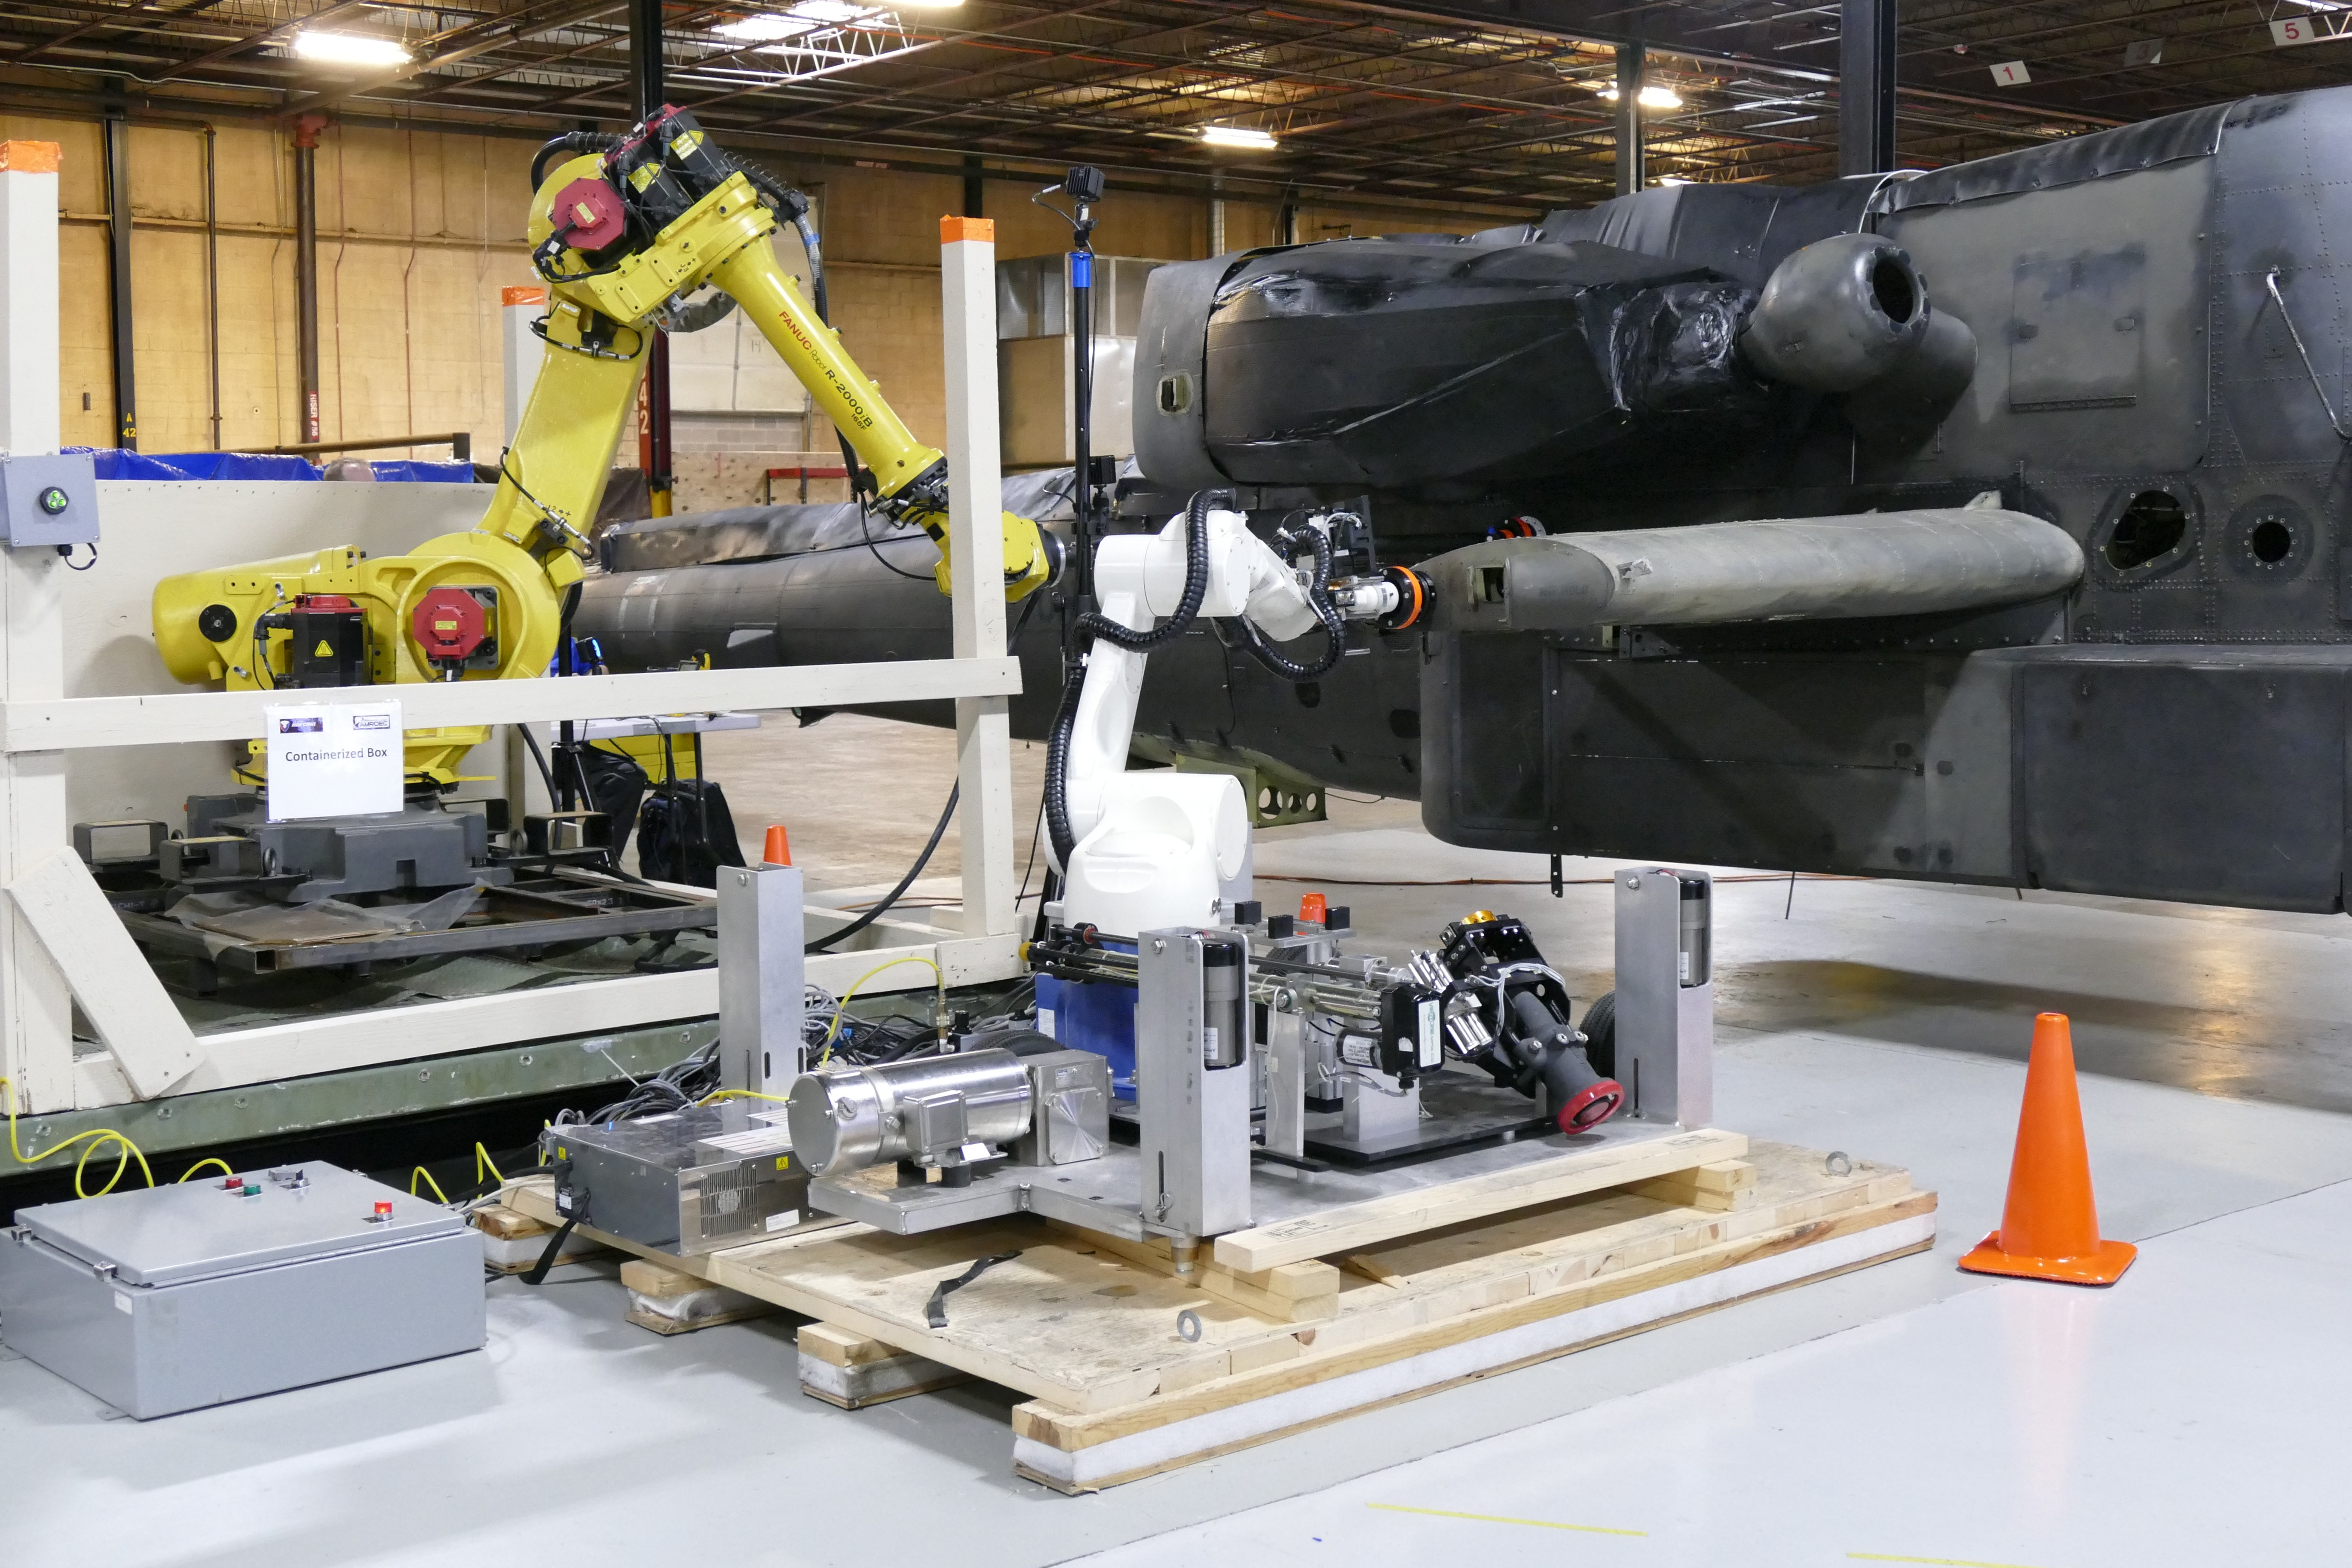
\includegraphics[width=0.5\textwidth]{figures/test_2017.jpg}
    \caption{AR3P Concept Development Prototype Robot (Photo Credit: U.S. Army)}\label{fig:test-2017}
\end{figure}

The AR3P project exemplifies the intersection of advanced robotics and
practical military applications, highlighting the potential of automated
systems to transform operational paradigms.
Figure~\ref{fig:automated-refuelling-systems} provides visual insights into the
capabilities of the AR3P system, by performing autonomous hot refuelling.
During this test, the robot is equipped with a LIDAR sensor and a camera to
detect the aircraft's refuelling port. In Figure~\ref{test-2020-2}, the AR3P
robot is seen approaching a detected aircraft, demonstrating its autonomous
navigation and alignment capabilities. In Figure~\ref{test-2020-3}, the AR3P
robot is shown engaging the aircraft refuelling port, emphasising its precision
and functionality in connecting to the aircraft’s fuel port. These images
illustrate the practical implementation of robotic technologies in enhancing
the safety, efficiency, and speed of refuelling operations, particularly in
challenging and hazardous environments \cite{AR3P2020}.

\begin{figure}[H]
    \centering
    \begin{subfigure}[b]{0.45\textwidth}
        \includegraphics[height=0.68\textwidth, width=\textwidth]{figures/test_2020_2.png}
        \caption{AR3P Robot Approaching Detected Aircraft (Photo Credit: Stratom)}\label{test-2020-2}
    \end{subfigure}
    \hfill
    \begin{subfigure}[b]{0.45\textwidth}
        \includegraphics[height=0.68\textwidth, width=\textwidth]{figures/test_2020_3.jpg}
        \caption{AR3P Robot Engaging Aircraft Refueling Port (Photo Credit: Stratom)}\label{test-2020-3}
    \end{subfigure}
    \caption{AR3P Robot Hot Refueling Demonstration for S-70 Helicopter}\label{fig:automated-refuelling-systems}
\end{figure}

\newpage

Unfortunately, there is very little literature on existing AAGR systems, as
most research is carried out by the military and is classified. The most recent
papers cover Autonomous Aerial Refueling (AAR) systems, which are used to
refuel unmanned aerial vehicles (UAVs) in mid-air. These systems are designed
to extend the flight time and range of UAVs by enabling them to refuel without
landing. AAR systems are particularly challenging due to the high speeds and
altitudes involved, as well as the need for precise measurement and tracking of
the relative position between the receiver aircraft and the tanker aircraft are
critical, particularly during the docking phase (see
figure~\ref{fig:aerial-refuelling})~\cite{AARBinocularVision,
    AARCNN}.~\citet{AAREKF} propose a robust solution that utilises monocular
vision combined with an extended Kalman filter (EKF) to address this challenge.
By implementing EKF, the system can provide reliable position estimations and
track the drogue within a specified region of interest (ROI), even in the
presence of disturbances such as air turbulence. As shown in
figure~\ref{fig:detection-system-aarekf}, this system initialises the state and
covariance matrices, predicts the drogue's position, updates the state based on
new measurements, and continuously refines the ROI for subsequent image
processing. This approach significantly reduces the processing time and
improves the detection frequency from 10 Hz to up to 30 Hz by focusing
computational resources on the predicted ROI. 

\begin{figure}[H]
    \centering
    \includegraphics[width=0.5\textwidth]{figures/x-47brefueling.jpg}
    \caption{Autonomous Aerial Refueling (AAR) of X-47B Unmanned Combat Air System Demonstrator (Photo Credit: U.S. Navy)}\label{fig:aerial-refuelling}
\end{figure}

\begin{figure}[H]
    \centering
    \includegraphics[width=0.6\textwidth]{figures/detection_system_AAREKF.png}
    \caption{Autonomous Air Refueling Detection System with EKF. Source: \citet{AAREKF}}\label{fig:detection-system-aarekf}
\end{figure}

\newpage
Recent advancements in autonomous ground refuelling have been driven by
improvements in computer vision and robotics.~\citet{AGRPoseEstimation}
presented the PosEst system, which combines 2D RGB images with 3D point cloud
data to enhance detection accuracy. This system uses a custom-trained
EfficientNet-B0 CNN for object detection and leverages the Kalman filter for
stable 3D pose estimation (see Figure~\ref{fig:agr-pose-kalman}). The PosEst
method employs a dual approach of high-precision detection and robust tracking.
By predicting and updating the object’s state in real-time, the Kalman filter
facilitates continuous and precise alignment of the fuel nozzle with the
refuelling adaptor, even in dynamic environments. This approach significantly
reduces the risks associated with manual refuelling and improves operational
efficiency and safety.

\begin{figure}[H]
    \centering
    \includegraphics[width=0.45\textwidth]{figures/AGRPoseKalman.png}
    \caption{Kalman Filter Workflow for Pose Estimation in Autonomous Ground Refueling. Source: \citet{AGRPoseEstimation}}\label{fig:agr-pose-kalman}
\end{figure}

One of the primary challenges in AAGR is the accurate detection and positioning
of the refuelling port under varying environmental conditions. Robust datasets
for scene recognition and machine learning applications have been developed to
address these challenges.~\citet{DatasetAGR} introduced a comprehensive dataset
for AAGR, addressing significant challenges such as variant illumination
conditions, different refuelling port types, and environmental obstructions.
The dataset comprises over 26,000 labeled images collected through image
crawling from 13 different databases, followed by augmentation to ensure
diversity (see Figure~\ref{fig:agr-dataset}). Additionally, recent innovations
have introduced hybrid datasets combining real and synthetic data for training
and validating systems \cite{HybridDatasetAGRV1}. This approach offers a wide
range of scenarios and conditions, improving the robustness and accuracy of
automated refuelling systems. The development of high-quality datasets is
pivotal in improving the robustness and reliability of AAGR systems.

\begin{figure}[H]
    \centering
    \includegraphics[width=0.4\textwidth]{figures/AGRDatasetGrid.png}
    \caption{AAGR Dataset Overview. Source: \citet{DatasetAGR}}\label{fig:agr-dataset}
\end{figure}

%%%%%%%%%%%%%%%%%%%%%%%%%%%%%%%%%%%%%%%%%%%%%%%%%%%%%%%%%%%%%%%%%%%%%%%%%%%%%%%%

\newpage
\section{Object Detection and Tracking in Computer Vision}
In Computer Vision, Object Detection refers to the identification and location
of individual objects within an image, providing both spatial information
(bounding boxes) and confidence scores, which represent the probability that
each detected object belongs to the predicted
class~\cite{huggingface2023objectdetection}. For example, in the following
image, there are five detections, including one `ball' with a confidence level
of 98\% and four `people' with confidence levels of 98\%, 95\%, 97\% and 97\%.

\begin{figure}[H]
    \centering
    \includegraphics[width=0.3\textwidth]{figures/intro_object_detection.png}
    \caption{Example of outputs from an object detector~\cite{huggingface2023objectdetection}.}\label{fig:object-detection}
\end{figure}

Over the last few decades, Object Detection models based on Deep Learning have
enjoyed remarkable success. These models fall into two main categories:
two-stage detectors and single-stage detectors. On the one hand, two-stage
detectors, such as R-CNN~\cite{DBLP:journals/corr/GirshickDDM13}, Fast
R-CNN~\cite{DBLP:journals/corr/Girshick15}, Faster R-CNN~\cite{Ren2017} and
R-FCN~\cite{DBLP:journals/corr/DaiLHS16}, first generate region proposals and
then refine these proposals into precise anchor boxes. While these models excel
in detection accuracy, they typically suffer from large model sizes and slower
detection speeds~\cite{SurveyDLOD, ODNetworkUAVCNNTransformer}. On the other
hand, single-stage detectors, including the SSD (Single Shot Multibox
Detector)~\cite{DBLP:journals/corr/LiuAESR15}, YOLO (You Only Look Once)
series~\cite{DBLP:journals/corr/RedmonDGF15, DBLP:journals/corr/RedmonF16,
    DBLP:journals/corr/abs-2004-10934, chen2023yoloms,
    DBLP:journals/corr/abs-2107-08430, YOLOv5Release, li2023yolov6, YOLOv8,
    wang2024yolov9, xu2022ppyoloe, wang2023goldyolo, xu2023damoyolo,
    wang2024yolov10}, and RetinaNet~\cite{lin2018focal} directly predict object
locations and categories in a single network pass. These models are known for
their high detection speeds but sometimes compromise accuracy~\cite{SurveyDLOD,
    ODNetworkUAVCNNTransformer}.

\begin{figure}[H]
    \centering
    \includegraphics[width=0.8\textwidth]{figures/one-stage_two-stage_OD.png}
    \caption{Basic deep learning-based one-stage vs two-stage object detection model architectures~\cite{SurveyDLOD}.}\label{fig:two-stage-vs-single-stage}
\end{figure}

\newpage
YOLOv10, the latest iteration in the YOLO series, marks a significant leap
forward in real-time object detection with the introduction of NMS-free
training. Traditionally, single-stage detectors relied on Non-Maximum
Suppression (NMS) during post-processing to eliminate redundant predictions, as
illustrated in Figure~\ref{fig:nms}. However, this process can sometimes be
overly aggressive, risking the loss of valuable predictions or failing to
remove all duplicates effectively, which also adds to computational costs
during both training and inference~\cite{LearnOpenCVYOLOv10}.

\begin{figure}[H]
    \centering
    \includegraphics[width=0.5\textwidth]{figures/NMS.png}
    \caption{Non-Maximum Suppression (NMS) in Object Detection~\cite{LearnOpenCVYOLOv10}.}\label{fig:nms}
\end{figure}

YOLOv10 overcomes these limitations by implementing a consistent dual
assignments strategy that facilitates NMS-free training. This strategy
leverages both one-to-many and one-to-one label assignments during training,
providing the model with rich supervision while enabling efficient end-to-end
deployment. During inference, the one-to-one assignment head is employed, which
eliminates the need for NMS and significantly reduces inference time. As
depicted in Figure~\ref{fig:yolov10}, the one-to-many head assigns multiple
labels to each anchor box, enriching the model’s supervision, while the
one-to-one head refines these predictions by assigning a single label to each
anchor box, ensuring precise and efficient detection~\cite{wang2024yolov10}.

\begin{figure}[H]
    \centering
    \includegraphics[width=0.5\textwidth]{figures/YOLOV10.png}
    \caption{YOLOv10 Model Workflow~\cite{wang2024yolov10}}\label{fig:yolov10}
\end{figure}

In addition, YOLOv10 adopts a holistic efficiency-accuracy driven design that
optimises the model’s architecture across various dimensions. The
classification head has been redesigned to be more lightweight, reducing
computational overhead while maintaining accuracy. The spatial-channel
decoupled downsampling technique separates spatial reduction and channel
increase operations, which lowers computational costs and reduces the parameter
count. Furthermore, the rank-guided block design minimises redundancy within
the model by adapting the complexity of different stages based on their
intrinsic rank values, ensuring optimal capacity-efficiency trade-offs. YOLOv10
also introduces large-kernel (see figure~\ref{fig:large-kernel-yolov10})
convolutions selectively in the deeper stages of the network to increase the
receptive field, allowing the model to capture more contextual information
without a significant increase in computational cost. Moreover, YOLOv10
incorporates a partial self-attention (PSA) mechanism, which integrates the
benefits of global context modeling while maintaining a lightweight
architecture. This careful balance of efficiency and accuracy enables YOLOv10
to deliver state-of-the-art
performance~\cite{wang2024yolov10,LearnOpenCVYOLOv10}.

\begin{figure}[H]
    \centering
    \includegraphics[width=0.5\textwidth]{figures/KernelYOLOv10.png}
    \caption{Large-Kernel Convolution in YOLOv10~\cite{LearnOpenCVYOLOv10}}\label{fig:large-kernel-yolov10}
\end{figure}

As shown in table~\ref{tab:yolov10-benchmarks}, extensive testing on standard
benchmarks, such as COCO, demonstrates YOLOv10’s superior performance in both
speed and accuracy. For example, YOLOv10-S is 1.8 times faster than RT-DETR-R18
while also using fewer parameters. Similarly, YOLOv10-B achieves a 46\%
reduction in latency compared to YOLOv9-C without compromising performance.
These results underscore YOLOv10’s effectiveness as a real-time end-to-end
object detection model, making it well-suited for applications requiring both
high speed and accuracy.

\begin{table}[H]
    \centering
    \caption{Performance Comparison of YOLO Models with State-of-the-Art Techniques. Latency is reported using official pre-trained models. \textsuperscript{f}Latency refers to the forward pass duration without including post-processing. \textsuperscript{\textdagger} indicates YOLOv10 results obtained with the original one-to-many training and Non-Maximum Suppression (NMS)~\cite{wang2024yolov10}.}
    \begin{adjustbox}{max width=\textwidth}
        \begin{tabular}{lcccccc}
            \toprule
            \textbf{Model}     & \textbf{Params (M)} & \textbf{FLOPs (G)} & \textbf{AP\textsubscript{val} (\%)}               & \textbf{Latency\textsuperscript{c} (ms)} & \textbf{Latency\textsuperscript{f} (ms)} \\
            \midrule
            YOLOv6-3.0-N       & 4.7                 & 11.4               & 37.0                                              & 2.69                                     & 1.76                                     \\
            Gold-YOLO-N        & 5.6                 & 12.1               & 39.6                                              & 2.92                                     & 1.82                                     \\
            YOLOv8-N           & 3.2                 & 8.7                & 37.3                                              & 6.16                                     & 1.77                                     \\
            \textbf{YOLOv10-N} & \textbf{2.3}        & \textbf{6.7}       & \textbf{38.5 / 39.5\textsuperscript{\textdagger}} & \textbf{1.84}                            & \textbf{1.79}                            \\  
            \midrule
            YOLOv6-3.0-S       & 18.5                & 45.3               & 44.3                                              & 3.42                                     & 2.35                                     \\  
            Gold-YOLO-S        & 21.5                & 46.0               & 45.4                                              & 3.82                                     & 2.73                                     \\  
            YOLO-MS-XS         & 4.5                 & 17.4               & 43.4                                              & 8.23                                     & 2.80                                     \\  
            YOLO-MS-S          & 8.1                 & 31.2               & 46.2                                              & 10.12                                    & 4.83                                     \\  
            YOLOv8-S           & 11.2                & 28.6               & 44.9                                              & 7.07                                     & 2.33                                     \\  
            YOLOv9-S           & 7.1                 & 26.4               & 46.7                                              & -                                        & -                                        \\  
            RT-DETR-R18        & 20.0                & 60.0               & 46.5                                              & 4.58                                     & 4.49                                     \\  
            \textbf{YOLOv10-S} & \textbf{7.2}        & \textbf{21.6}      & \textbf{46.3 / 46.8\textsuperscript{\textdagger}} & \textbf{2.49}                            & \textbf{2.39}                            \\  
            \midrule
            YOLOv6-3.0-M       & 34.9                & 85.8               & 49.1                                              & 5.63                                     & 4.56                                     \\  
            Gold-YOLO-M        & 41.3                & 87.5               & 49.8                                              & 6.38                                     & 5.45                                     \\  
            YOLO-MS            & 22.2                & 80.2               & 51.0                                              & 12.41                                    & 7.30                                     \\  
            YOLOv8-M           & 25.9                & 78.9               & 50.6                                              & 9.50                                     & 5.09                                     \\  
            YOLOv9-M           & 20.0                & 76.3               & 51.1                                              & -                                        & -                                        \\  
            RT-DETR-R34        & 31.0                & 92.0               & 48.9                                              & 6.32                                     & 6.21                                     \\  
            RT-DETR-R50m       & 36.0                & 100.0              & 51.3                                              & 6.90                                     & 6.84                                     \\  
            \textbf{YOLOv10-M} & \textbf{15.4}       & \textbf{59.1}      & \textbf{51.1 / 51.3\textsuperscript{\textdagger}} & \textbf{4.74}                            & \textbf{4.63}                            \\  
            \bottomrule
        \end{tabular}
    \end{adjustbox}
    \label{tab:yolov10-benchmarks}
\end{table}

Evaluating Object Detection models involves several key metrics to measure
their performance. One common metric is Intersection over Union (IoU), which
measures the overlap between a predicted bounding box and a ground-truth
bounding box, as shown in Figure~\ref{fig:iou-metric}.

\begin{figure}[H]
    \centering
    \includegraphics[width=0.8\textwidth]{figures/iou.png}
    \caption{Intersection over Union (IoU) between a detection (in green) and ground-truth (in blue).~\cite{huggingface2023objectdetection}}\label{fig:iou-metric}
\end{figure}

Based on the IoU metric, a detection can be classified as a \textbf{True
    Positive (TP)} or a \textbf{False Positive (FP)} depending on whether the IoU
value exceeds a certain threshold ($T_{IoU}$). If the IoU is above the
threshold, the detection is considered correct (TP); otherwise, it is
classified as a False Positive (FP). Additionally, \textbf{False Negatives
    (FN)} refer to ground truth objects not detected by the model, while
\textbf{True Negatives (TN)} are correctly classified background
detections~\cite{huggingface2023objectdetection}. These classifications allow
for the calculation of the following metrics:

\begin{itemize}
    \item \textbf{Precision}: The ratio of True Positives to the total number of
          detections, measuring the model's ability to avoid false positives:
          \begin{equation}
              \text{Precision} = \frac{\text{TP}}{\text{TP} + \text{FP}}
          \end{equation}

    \item \textbf{Recall}: The ratio of True Positives to the total number of ground-truth objects, measuring the model's ability to avoid false negatives:
          \begin{equation}
              \text{Recall} = \frac{\text{TP}}{\text{TP} + \text{FN}}
          \end{equation}
\end{itemize}

Common metrics used to evaluate Object Detection include:

\begin{itemize}
    \item \textbf{Average Precision (AP)}: This combines precision and recall, providing a single figure summarizing the model's performance across different confidence thresholds. Common versions are AP@.5 (with a threshold of 0.5 IoU) and AP@[.5:.05:.95], which calculates the average of AP values over several IoU thresholds~\cite{huggingface2023objectdetection}.
    \item \textbf{Average Recall (AR)}: This measures the recall of the model averaged across multiple IoU thresholds. It can be computed for different numbers of detections per image, such as AR@1, AR@10, etc.~\cite{huggingface2023objectdetection}.
    \item \textbf{Inference Time}: The time taken by the model to process an image, which is critical for applications requiring real-time detection~\cite{huggingface2023objectdetection}.
    \item \textbf{Model Size}: The number of parameters or the size of the model, affecting deployment, especially on devices with limited resources~\cite{huggingface2023objectdetection}.
    \item \textbf{Efficiency}: This considers the trade-off between accuracy and speed, often visualized using the AP vs. inference time curve~\cite{huggingface2023objectdetection}.
\end{itemize}

In addition to Object Detection, Object Tracking is another critical task in
Computer Vision, involving the continuous monitoring of objects across video
frames. Object Tracking methods can be broadly classified into two categories:
\textbf{Generative Trackers} and \textbf{Discriminative
    Trackers}~\cite{SurveyVisualOT}. Generative trackers are capable of handling
challenging scenarios such as occlusion and large-scale variation through
particle sampling strategies, often integrated with various appearance models,
including sparse representation and energy of motion. Discriminative trackers,
by contrast, build robust classifiers using hand-crafted or deep
features~\cite{SurveyVisualOT}. The combination of generative and
discriminative approaches, as well as the integration of deep learning
techniques such as fully revolutionary networks and Transformer models, has led
to significant improvements in object detection
performance~\cite{OverviewCorrelationAlgoOT, SuveyAdvancesSingleOTMethods,
    SurveyModernODModels}. In addition, the speed and computational requirements of
these algorithms are critical factors influencing their practical
applicability~\cite{SuveyAdvancesSingleOTMethods, SurveyModernODModels,
    SurveyTransformersSingleOT}. Advanced techniques in object tracking leverage
both generative and discriminative models to amplify tracking efficacy. The
utilisation of deep trackers has evidenced superior results on public tracking
datasets, attributed to their potent feature extractors, accurate bounding box
regressors, and discriminative classifiers~\cite{SurveyTransformersSingleOT}.
Techniques such as deformable convolution and Transformer models extend
traditional convolution or correlation methodologies to execute global feature
matching, thereby enhancing tracking accuracy. The incorporation of contextual
or knowledge information can substantially elevate performance, with
methodologies like Particle Filtering, also recognised as Sequential Monte
Carlo (SMC) methods, framed as problems of Bayesian inference in state
space~\cite{SurveySmallObjectDetection, SmallObjectDetectionPositonPrediction}.
The extended Kalman Filtering (EKF) is another advanced technique that has been
employed to improve tracking accuracy by predicting the current status through
the previous status and modifying the prediction result based on observation
information~\cite{SuveyAdvancesSingleOTMethods, SurveyModernODModels}. Despite
these advancements, the integration of these methods in a complementary manner
remains an open research area with substantial potential for advancing the
field~\cite{OverviewCorrelationAlgoOT, SuveyAdvancesSingleOTMethods}.

\newpage
\section{Deep Learning for Spacio-Temporal Prediction}
Time series prediction involves processing sequential data to predict future
events or values. Various deep learning models have been applied to this task,
requiring several preparatory steps such as collecting data, designating
attribute types, dealing with inconsistencies and storing datasets. These
datasets are usually classified into units of time such as seconds, minutes and
hours, allowing the construction of metadata for machine
learning~\cite{FFPSpaceSystemVehicles}.

\subsection*{Deep Learning Sequence Models}
The problem of predicting the future locations of objects has been extensively
studied, particularly for static surveillance cameras. Initial efforts utilised
recurrent neural networks (RNNs), including long-term memory networks (LSTMs)
and gated recurrent units (GRUs), in an encoder-decoder format to encode past
observations and decode future locations. 

Recurrent Neural Networks (RNNs), particularly Long Short-Term Memory networks
(LSTMs) and Gated Recurrent Units (GRUs), have exhibited promise in this
direction. Nevertheless, most RNN-based models suffer from performance
degradation over time since they rely on recurrently predicting future bounding
boxes based on previous outputs. 

\begin{figure}[H]
    \centering
    \includegraphics[width=0.6\textwidth]{figures/lstm-rnn-gru.png}
    \caption{Comparing different Sequence models: RNN, LSTM, and GRU. Source: Colah's blog. Compiled by AIML.com}\label{fig:lstm-rnn-gru}
\end{figure}

Early models integrated additional inputs such as environmental data and
semantic actions to enhance prediction accuracy. For
instance,~\citet{Alahi2016} proposed a Social-LSTM to model pedestrian
trajectories and interactions, further improving global context capture through
a social pooling module.

\subsection*{Deep Learning for Spatio-Temporal Prediction}
\subsubsection*{STED Model}

The STED (Spatio-Temporal Encoder-Decoder) model was introduced
by~\citet{MultipleObjectForecasting} as a novel approach for multiple object
forecasting (MOF), particularly in predicting the future bounding boxes of
tracked objects from video sequences. This model is designed to handle the
challenges of object forecasting in diverse environments, leveraging both
visual and temporal features to predict object-motion and ego-motion
effectively. As shown in figure~\ref{fig:sted}, the STED model consists of
three main components: a bounding box feature encoder, an optical flow feature
encoder, and a decoder. The \textit{Bounding Box Feature Encoder} utilises a
Gated Recurrent Unit (GRU) to extract temporal features from past object
bounding boxes, which include coordinates $(x, y)$, dimensions $(w, h)$, and
velocity changes $(\Delta x, \Delta y, \Delta w, \Delta h)$ over a window of 30
frames, representing 1 second of observation. Simultaneously, the
\textit{Optical Flow Feature Encoder} captures motion features directly from
optical flow, using a Convolutional Neural Network (CNN) to process a stack of
10 frames sampled uniformly from the past 1 second of video data. The
combination of these features provides a comprehensive understanding of both
the object's movement and the camera's movement (ego-motion). The
\textit{Decoder} then takes the concatenated feature vector from the encoders
and predicts the future bounding box coordinates for the next 60 frames (2
seconds prediction window). The GRU-based decoder generates bounding box
predictions iteratively, using the encoded feature vector and the internal
hidden state to output changes in bounding box velocity and dimensions over
time.

\begin{figure}[H]
    \centering
    \includegraphics[width=1\textwidth]{figures/STED.png}
    \caption{STED Model Architecture. Source:~\citet{MultipleObjectForecasting}}\label{fig:sted}
\end{figure}

The STED architecture is specifically designed to address the complexities of
predicting future object positions in video sequences, particularly under
conditions of non-linear object motion and varying scales due to camera
movement. By combining temporal features from bounding boxes with motion
information from optical flow, the model effectively captures both the dynamic
behavior of the objects and the impact of the camera's motion on the observed
scene. The STED model was evaluated on the Citywalks dataset, a diverse dataset
designed to test the model's ability to predict future object locations across
different environments. The performance of STED was compared with several
baseline models, as summarised in Table~\ref{tab:sted-results}.

\begin{table}[H]
    \centering
    \caption{Comparison of the performance of STED with baseline models on the Citywalks dataset. Metrics include Average Displacement Error (ADE), Final Displacement Error (FDE), Average Intersection-over-Union (AIoU), and Final Intersection-over-Union (FIoU). The model was evaluated using 1 second of input frames to predict 2 seconds of future frames.}
    \begin{adjustbox}{max width=\textwidth}
        \begin{tabular}{lcccc}
            \toprule
            \textbf{Model}                         & \textbf{ADE (pixels)} & \textbf{FDE (pixels)} & \textbf{AIoU (\%)} & \textbf{FIoU (\%)} \\ 
            \midrule
            CV-CS~\cite{MultipleObjectForecasting} & 31.6                  & 57.6                  & 46.0               & 21.3               \\
            LKF~\cite{MultipleObjectForecasting}   & 32.9                  & 59.0                  & 43.9               & 20.1               \\
            STED~\cite{MultipleObjectForecasting}  & \textbf{26.0}         & \textbf{46.9}         & \textbf{51.8}      & \textbf{27.5}      \\
            \bottomrule
        \end{tabular}
    \end{adjustbox}
    \label{tab:sted-results}
\end{table}

The STED model achieved an Average Displacement Error (ADE) of 26.0 pixels and
a Final Displacement Error (FDE) of 46.9 pixels, with an Average Intersection
Over Union (AIoU) of 51.8\% and a Final Intersection Over Union (FIoU) of
27.5\%. These results indicate that STED outperforms existing models in both
displacement and intersection-over-union metrics, making it a robust solution
for forecasting future object locations in challenging video sequences.

In summary, the STED model’s ability to combine visual and temporal features
from both object bounding boxes and optical flow enables it to predict future
object positions more accurately, making it an effective tool for applications
in autonomous driving and robotic navigation.

\subsubsection*{PV-LSTM Model}

The PV-LSTM (Position-Velocity Long Short-Term Memory) model was developed
by~\citet{DBLP:journals/corr/abs-2010-10270} to predict pedestrian intentions
and future bounding box positions, a crucial task for enhancing the safety of
autonomous driving systems. The architecture of this model is illustrated in
figure~\ref{fig:pv-lstm}. The model utilises a sequence-to-sequence LSTM
architecture that processes both spatial and temporal information effectively.
To do that, it processes input sequences of observed bounding boxes $(x, y, w,
    h)$ and their velocity changes $(\Delta x, \Delta y, \Delta w, \Delta h)$ over
a window of 30 frames, representing 1 second of observation. These inputs are
encoded through two encoders: the \textit{Bounding Box Position Encoder} and
the \textit{Bounding Box Velocity Encoder}. The encoded features are then
concatenated and passed to two decoders: the \textit{Velocity Decoder}, which
predicts future bounding box velocities, and the \textit{Intention Decoder},
which predicts pedestrian crossing intentions over the next 60 frames (2
seconds prediction window). The PV-LSTM model’s architecture is designed to
capture the dynamic and complex nature of pedestrian behavior, which is crucial
for real-time decision-making in autonomous driving. By integrating both
position and velocity information through dual encoders, the model can more
accurately predict the future movements and intentions of pedestrians, thus
enhancing safety and reliability in autonomous navigation systems.

\begin{figure}[H]
    \centering
    \includegraphics[width=1\textwidth]{figures/PV-LSTM.png}
    \caption{PV-LSTM Model Architecture. Source:~\citet{DBLP:journals/corr/abs-2010-10270}}\label{fig:pv-lstm}
\end{figure}

The PV-LSTM model was evaluated on the Citywalks dataset, and its performance
was compared against several baseline models. The results are summarised in
Table~\ref{tab:pv-lstm-results}, showcasing the model's effectiveness in
predicting pedestrian trajectories and intentions. The PV-LSTM model achieved
an Average Displacement Error (ADE) of 25.2 pixels and a Final Displacement
Error (FDE) of 49.9 pixels, with an Average Intersection Over Union (AIoU) of
40.2\%. Although the STED model slightly outperforms in AIoU and FIoU, the
PV-LSTM model provides a robust solution with competitive prediction accuracy,
while maintaining a simpler architecture.

\begin{table}[H]
    \centering
    \caption{Comparison of the performance of PV-LSTM with baseline models on the Citywalks dataset. Metrics include Average Displacement Error (ADE), Final Displacement Error (FDE), and Average Intersection-over-Union (AIoU). The model was evaluated using 1 second of input frames to predict 2 seconds of future frames.}
    \begin{adjustbox}{max width=\textwidth}
        \begin{tabular}{lcccc}
            \toprule
            \textbf{Model}                                   & \textbf{ADE (pixels)} & \textbf{FDE (pixels)} & \textbf{AIoU (\%)} & \textbf{FIoU (\%)} \\ 
            \midrule
            CV-CS~\cite{DBLP:journals/corr/abs-2010-10270}   & 31.6                  & 57.6                  & 46.0               & 21.3               \\
            LKF~\cite{DBLP:journals/corr/abs-2010-10270}     & 32.9                  & 59.0                  & 43.9               & 20.1               \\
            STED~\cite{DBLP:journals/corr/abs-2010-10270}    & \textbf{26.0}         & \textbf{46.9}         & \textbf{51.8}      & \textbf{27.5}      \\
            PV-LSTM~\cite{DBLP:journals/corr/abs-2010-10270} & 25.2                  & 49.9                  & 40.2               & 20.3               \\
            \bottomrule
        \end{tabular}
    \end{adjustbox}
    \label{tab:pv-lstm-results}
\end{table}

\subsubsection*{Fusion-GRU Model}

\citet{FusionGRU} developed the Fusion-Gated Recurrent
Unit (Fusion-GRU) model to predict the future bounding boxes of traffic agents
in risky driving scenarios. This model leverages multiple sources of
information, such as location-scale data, monocular depth information, and
optical flow data, to capture complex interactions among these cues and
transform them into meaningful hidden representations. This approach is
particularly suited for dealing with scenarios where the available observation
time is limited due to abrupt motion changes or tracking loss. 
The Fusion-GRU model consists of several components that work together to
predict future bounding boxes. The model takes input video sequences, extracts
depth maps, and calculates optical flow to capture motion dynamics. Bounding
boxes are detected and tracked using YOLOv5 and DeepSort, respectively. The
feature extractor processes both object-level and scene-level features using
ResNet50, transforming them into feature vectors. These vectors are then
concatenated and passed to the Fusion-GRU encoder, which integrates location,
scale, and distance information into hidden representations. 
The model also introduces an intermediary estimator, which generates
intermediate bounding boxes that help in capturing sequential dependencies
across frames. Additionally, a self-attention aggregation layer is employed to
reduce error accumulation by focusing on the most relevant information for
long-term predictions. Finally, a GRU decoder iteratively predicts the future
bounding boxes based on the aggregated feature vectors and the hidden
representations from the Fusion-GRU encoder.

\begin{figure}[H]
    \centering
    \includegraphics[width=1\textwidth]{figures/FusionGRU.png}
    \caption{Fusion-GRU model architecture. Source:~\citet{FusionGRU}}\label{fig:fusion-gru}
\end{figure}

The Fusion-GRU model is specifically designed to address the limitations of
traditional GRU-based models, which often suffer from performance degradation
over time. By integrating complex interactions among various input features and
employing self-attention mechanisms, the Fusion-GRU model enhances its ability
to predict future bounding boxes more accurately. This architecture is
particularly effective in cluttered and dynamic driving environments, where
understanding the relationships between different traffic agents and their
surroundings is crucial for accurate prediction.

The Fusion-GRU model was evaluated on two publicly available datasets, ROL
(Risky Object Localization) and HEV-I (Honda Egocentric View-Intersection),
demonstrating its superior performance in predicting future bounding boxes
compared to other state-of-the-art models. The results are summarised in
Table~\ref{tab:fusion-gru-results}, which compares the performance of
Fusion-GRU with baseline models based on metrics such as Average Displacement
Error (ADE), Final Displacement Error (FDE), and Intersection over Union (IOU).

\begin{table}[H]
    \centering
    \caption{Comparison of the performance of Fusion-GRU with baseline models on the ROL and HEV-I datasets. Metrics include ADE, FDE, and FIoU. The model was evaluated using 0.5-second and 1-second prediction horizons.}
    \begin{adjustbox}{max width=\textwidth}
        \begin{tabular}{lcccc}
            \toprule
            \textbf{Model}              & \textbf{ADE0.5 (pixels)} & \textbf{FDE0.5 (pixels)} & \textbf{FIoU0.5 (\%)} & \textbf{ADE1.0 (pixels)} \\ 
            \midrule
            FOL-X~\cite{FusionGRU}      & 6.7                      & 11.0                     & 85.0                  & 12.6                     \\
            SGDNet~\cite{FusionGRU}     & 6.3                      & --                       & --                    & 11.4                     \\
            Fusion-GRU~\cite{FusionGRU} & \textbf{5.5}             & \textbf{8.3}             & \textbf{85.2}         & \textbf{11.2}            \\
            \bottomrule
        \end{tabular}
    \end{adjustbox}
    \label{tab:fusion-gru-results}
\end{table}

The Fusion-GRU model achieved the lowest Average Displacement Error (ADE) and
Final Displacement Error (FDE) in both 0.5-second and 1-second prediction
horizons on the HEV-I dataset. It also exhibited the highest Final Intersection
over Union (FIoU) of 85.2\% in the 0.5-second horizon, indicating its strong
capability to accurately predict the future positions and scales of traffic
agents.

%%%%%%%%%%%%%%%%%%%%%%%%%%%%%%%%%%%%%%%%%%%%%%%%%%%%%%%%%%%%%%%%%%%%%%%%%%%%%%%
%%%%%%%%%%%%%%%%%%%%%%%%%%%%%%%%% METHODOLOGY %%%%%%%%%%%%%%%%%%%%%%%%%%%%%%%%%
\chapter{Methodology}\label{chap:methodology}
\section{Dataset Configuration}
\subsection{Dataset Description}
The `Indoor Hangar Fueling Port Detection and Tracking Dataset' (HARD) is an
integral part of Phase-1 of the ONEHeart project, funded by UKRI. The ONEHeart
project aims to develop an automated aircraft refuelling system based on
computer vision and robotics technology. This dataset can be utilised for
various purposes, including but not limited to refueling port detection,
fueling port tracking, camera pose estimation, and visual image processing. It
is provided under the terms of the UKRI funding agreement. Unauthorised use,
distribution, or reproduction is prohibited. The HARD dataset consists of 21
video sequences captured in an indoor hangar at the Aerospace Integration
Research Centre (AIRC). The videos were recorded using an Intel®
${\text{RealSense}}^{\text{TM}}$ D435~\cite{IntelRealSense} (Shown in
Figure~\ref{fig:intel-realsense-d435}), which provides depth information in
addition to RGB data. The target area for detection and tracking is near the
refueling port of an Airbus A320 wing. The videos were recorded under different
lighting conditions, including indoor artificial lighting and natural daylight,
to simulate real-world scenarios. In addition, the refueling port was in
different states (closed, open, and semi-open) to capture a wide range of
variations for training and testing machine learning models.

\begin{figure}[H]
    \centering
    \includegraphics[width=0.8\textwidth]{figures/depth-camera-d435_details.jpg}
    \caption{Intel® ${\text{RealSense}}^{\text{TM}}$ D435 Depth Camera. Source: Intel}\label{fig:intel-realsense-d435}
\end{figure}

\newpage
\subsection{Data Annotation}
The HARD dataset provided for this project was not fully annotated. Therefore,
the first step in the data preparation process was to annotate the dataset.
This annotation process was crucial to enable the training of machine learning
models for accurate refueling port detection and tracking. Initially, 100
frames from each video sequence were manually annotated. This involved labeling
the refueling port in each frame, which required identifying and marking the
exact location of the refueling port using bounding boxes. This was done using
the Label Studio tool, a powerful annotation platform that allows users to
create and manage annotations in images and videos. Label Studio was chosen for
its flexibility and ease of use. It supports various annotation formats and
integrates well with machine learning workflows. Users can draw bounding boxes
around objects of interest, in this case, the refueling port, to create labeled
datasets. The initial manual annotations created a preliminary dataset. This
dataset was used to train a YOLOv10 (You Only Look Once, version 10) model for
refueling port detection. The annotated dataset was used to train the YOLOv10
model. The model learned to detect the refueling port from the annotated
images, improving its accuracy with each training iteration. After training the
YOLOv10 model, it was implemented as a backend service for Label Studio. This
was deployed as a Docker container, allowing the model to be used for automated
annotation of the remaining images in the dataset. The model predicted the
location of the refueling port in new frames, and these predictions were used
to annotate the rest of the dataset automatically. Each automatically generated
annotation was reviewed manually to ensure accuracy. This review process
involved verifying the location of the refueling port in each frame and making
necessary corrections to the annotations. This thorough quality control ensured
that the entire dataset was consistently and accurately labeled.This
comprehensive annotation process ensured that the entire dataset was accurately
labeled, providing a robust foundation for training machine learning models
aimed at refueling port detection and tracking. The combination of manual and
automated annotation techniques maximised efficiency while maintaining high
annotation quality. 

\newpage
\subsection{Summary of Available Videos}
Each video was assigned to a specific dataset (train, val, and test), with an
approximate split of 70\% for training, 15\% for validation, and 15\% for
testing. The following table presents the available videos in the dataset along
with the number of frames for each video and their assignment:

\begin{table}[H]
    \centering
    \begin{tabular}{@{}cccc@{}}
        \toprule
        \textbf{Type}      & \textbf{Video Name}                           & \textbf{Number of Frames} & \textbf{Assignment} \\ \midrule
        \textbf{Closed}    & \textbf{video\_lab\_platform\_1}              & \textbf{624}              & \textbf{train}      \\
        Closed             & video\_lab\_platform\_2                       & 639                       & train               \\
        Closed             & video\_lab\_platform\_5                       & 398                       & train               \\
        Closed             & video\_lab\_platform\_7                       & 412                       & train               \\
        Closed             & video\_lab\_platform\_8                       & 470                       & train               \\
        Closed             & video\_lab\_platform\_9                       & 373                       & train               \\
        Closed             & video\_lab\_manual\_1                         & 746                       & train               \\
        Closed             & video\_lab\_platform\_3                       & 569                       & val                 \\
        Closed             & video\_lab\_platform\_4                       & 247                       & val                 \\
        Closed             & video\_lab\_platform\_6                       & 303                       & test                \\
        Closed             & test\_outdoor1                                & 499                       & test                \\
        \textbf{Open}      & \textbf{video\_lab\_open\_1\_\_\_\_\_\_1}     & \textbf{497}              & \textbf{train}      \\
        Open               & video\_lab\_open\_1\_\_\_\_\_\_2              & 602                       & train               \\
        Open               & video\_lab\_open\_1\_\_\_\_\_\_3              & 313                       & train               \\
        Open               & video\_lab\_open\_1\_\_\_\_\_\_4              & 310                       & train               \\
        Open               & test\_indoor2                                 & 310                       & val                 \\
        Open               & test\_indoor1                                 & 314                       & test                \\
        \textbf{Semi-Open} & \textbf{video\_lab\_semiopen\_1\_\_\_\_\_\_1} & \textbf{739}              & \textbf{train}      \\
        Semi-Open          & video\_lab\_semiopen\_1\_\_\_\_\_\_2          & 439                       & train               \\
        Semi-Open          & video\_lab\_semiopen\_1\_\_\_\_\_\_4          & 372                       & val                 \\ 
        Semi-Open          & video\_lab\_semiopen\_1\_\_\_\_\_\_3          & 383                       & test                \\ \bottomrule
    \end{tabular}
    \caption{\centering Summary of available videos in the HARD dataset with their assignment.}
    \label{tab:video_summary}
\end{table}

\subsection{Data Distribution}
Before balancing the data, the distribution of video frames across the
different datasets (train, validation, and test) for each state of the fueling
port (CLOSED, OPEN, and SEMI-OPEN) was as follows:
\begin{table}[H]
    \centering
    \begin{tabular}{@{}ccccc@{}}
        \toprule
        \textbf{Type}      & \textbf{Total Frames} & \textbf{Train} & \textbf{Test} & \textbf{Validation} \\ \midrule
        \textbf{CLOSED}    & 5280                  & 3662 (69.36\%) & 802 (15.19\%) & 816 (15.45\%)       \\ 
        \textbf{OPEN}      & 2346                  & 1722 (73.40\%) & 314 (13.38\%) & 310 (13.21\%)       \\ 
        \textbf{SEMI-OPEN} & 1933                  & 1178 (60.94\%) & 383 (19.81\%) & 372 (19.24\%)       \\ \bottomrule
    \end{tabular}
    \caption{\centering Distribution of frames across train, test, and validation sets for each state in the HARD dataset before balancing.}
    \label{tab:frame_distribution}
\end{table}

As shown in~\ref{tab:frame_distribution}, the dataset initially had an
imbalance in the number of frames for each state. For instance, the CLOSED
state had significantly more frames compared to the OPEN and SEMI-OPEN states.
This imbalance could lead to biased training and inaccurate model performance,
as the model might become overly familiar with the more prevalent CLOSED state
and underperform on the less represented states.

\subsection{Balanced Data Distribution}
To address this issue, a balancing strategy was employed to create a more
uniform dataset. The first step involved shuffling and subsetting each state
(CLOSED, OPEN, and SEMI-OPEN) to keep only the minimum number of frames for
each state. This ensured that the number of frames for each state was equal,
avoiding bias towards any particular state. The subsets were then merged to
create three balanced datasets: Training, Validation, and Test, each with an
equal number of frames for each state. Finally, the balanced datasets were
shuffled again and resized to maintain the required split ratio of 70\% for
training, 15\% for validation, and 15\% for testing. The balanced dataset will
be used for training and evaluating the object detection model, while the full
dataset will be utilised for sequence model training and framework evaluation.
The resulting distribution of frames across the train, test, and validation
sets for each state after balancing is as follows:
\begin{table}[H]
    \centering
    \begin{tabular}{@{}cc@{}}
        \toprule
        \textbf{Dataset} & \textbf{Total Frames} \\ \midrule
        \textbf{Train}   & 3534 (69.57\%)        \\ 
        \textbf{Test}    & 773  (15.22\%)        \\ 
        \textbf{Val}     & 773  (15.22\%)        \\ \bottomrule
    \end{tabular}
    \caption{\centering Distribution of frames across train, test, and validation sets for each state in the HARD dataset after balancing.}
    \label{tab:balanced_frame_distribution}
\end{table}

The primary reason for balancing the dataset is to ensure that the object
detection model is equally trained on all states of the refueling port. An
imbalanced dataset could cause the model to perform well on the more common
states (like CLOSED) while underperforming on the less common states (like OPEN
and SEMI-OPEN). By balancing the dataset, the model has an equal opportunity to
learn from all states, improving its generalisation and robustness. This
strategy also prevents the model from becoming biased towards any particular
state, ensuring consistent performance across all states, which is critical for
the reliable operation of the automated refueling system.

\section{Framework Design}
The proposed framework, illustrated in Figure~\ref{fig:framework-workflow}, is
designed to predict the future positions of the refueling port’s bounding boxes
across the next \(m\) frames of a video stream. It does this by leveraging the
bounding boxes observed in the current and previous frames. At any given time
step \(t\), the observed bounding box is denoted as \(\mathbf{b}_t = [x_t, y_t,
w_t, h_t]\), where \((x_t, y_t)\) represents the center coordinates of the
bounding box, and \(w_t\) and \(h_t\) represent the width and height of the
bounding box, respectively. The goal is to predict a sequence of future
bounding boxes, \(\mathbf{S}_{t+1:t+m} = \{\mathbf{b}_{t+1}, \dots,
\mathbf{b}_{t+m}\}\), for the upcoming \(m\) frames based on the observed
bounding boxes from the past \(n\) frames, \(\mathbf{S}_{t-1+n:t} =
\{\mathbf{b}_{t-1+n}, \dots, \mathbf{b}_{t}\}\). 

\begin{figure}[H]
    \centering
    \includegraphics[width=0.79\textwidth]{figures/FrameworkWorkflow.drawio.pdf}
    \caption{Framework Workflow}\label{fig:framework-workflow}
\end{figure}

The process starts with an input video sequence, which is analysed on a
frame-by-frame basis. An object detection model first identifies and locates
the bounding boxes of the refueling port in each frame. These detected bounding
boxes are then formatted into input vectors suitable for the sequence model.
The sequence model is responsible for predicting the future spatial positions
and dimensions of the refueling port’s bounding boxes. Finally, these
predictions are refined through postprocessing steps to produce the final
bounding box forecasts for the subsequent frames.

\section{Object Detection Model Fine-tuning}
A fine-tuned YOLOv10 Nano model is used to detect the refueling port within the
video frames. As highlighted in the literature review, YOLOv10 represents the
latest advancement in object detection technology, offering an optimal balance
between speed and accuracy. The YOLOv10 Nano variant is particularly
well-suited for real-time applications, especially on resource-constrained
embedded devices, due to its lightweight architecture. The model is fine-tuned
through transfer learning on the HARD dataset, enabling precise detection of
the refueling port within the video frames. This fine-tuning process ensures
that the model meets the demands of real-time video analysis with both accuracy
and responsiveness. The implementation uses the Ultralytics YOLOv10 framework,
which provides a reliable and efficient pipeline for both training and
inference. This framework optimises detection performance and guarantees robust
operation in different scenarios.

\section{Sequence Model Design}
This thesis introduces the \textit{SizPos-GRU model} model, a deep learning
sequence model for predicting future positions and sizes of a unique object in
a video stream. The model leverages an encoder-attention-decoder architecture
to capture temporal dependencies and spatial relationships effectively. The
SizPos-GRU model leverages an encoder-attention-decoder architecture to
effectively capture temporal dependencies and spatial relationships. The
framework consists of four main components: two encoders, an attention
mechanism, and two decoders. Each component is designed to handle specific
aspects of the sequence modeling task, from encoding input sequences to
generating context-aware predictions.

\begin{figure}[H]
    \centering
    \includegraphics[width=1\textwidth]{figures/GRUSizPos.drawio.pdf}
    \caption{SizPos-GRU Model Architecture}\label{fig:sizpos-gru}
\end{figure}

\newpage
\subsection{Input Representation}
The \textit{SizPos-GRU} model expects two types of input sequences to predict
the future positions and sizes of an object. The first input captures the
spatial dynamics of the object, including its position, velocity and
acceleration. The second input focuses on the object's dimensional attributes,
such as its width and height, and changes in these dimensions over time.

\subsubsection*{Spatial Dynamics Vector}
The spatial dynamics vector at time $t$, denoted as $\mathbf{p}_t$, represents the position, velocity, and acceleration of the bounding box center. It is defined as:
\begin{align}
    \mathbf{p}_t & = \left(x_t, y_t, v_{x,t}, v_{y,t}, a_{x,t}, a_{y,t}\right), \\
    v_{x,t}      & = x_t - x_{t-1}, \quad v_{y,t} = y_t - y_{t-1},              \\
    a_{x,t}      & = v_{x,t} - v_{x,t-1}, \quad a_{y,t} = v_{y,t} - v_{y,t-1}.
\end{align}
Here, $(x_t, y_t)$ represents the center coordinates at time $t$, $(v_{x,t}, v_{y,t})$ are the velocities, and $(a_{x,t}, a_{y,t})$ are the accelerations along the $x$ and $y$ axes, respectively.

\subsubsection*{Dimensional Attributes Vector}
The dimensional attributes vector at time $t$, denoted as $\mathbf{d}_t$, captures the size of the bounding box and the changes in its dimensions:
\begin{align}
    \mathbf{d}_t & = \left(w_t, h_t, \Delta w_t, \Delta h_t\right),    \\
    \Delta w_t   & = w_t - w_{t-1}, \quad \Delta h_t = h_t - h_{t-1}.
\end{align}
Here, $(w_t, h_t)$ represents the width and height at time $t$, and $(\Delta w_t, \Delta h_t)$ are the changes in these dimensions from the previous time step.

\subsubsection*{Input Sequences for Model}
The sequences of these vectors over a time window of \(n\) frames are fed into the model as:
\[
    \mathbf{P} = \{\mathbf{p}_{t-1+n}, \mathbf{p}_{t-n+2}, \dots, \mathbf{p}_t\}, \quad \mathbf{D} = \{\mathbf{d}_{t-1+n}, \mathbf{d}_{t-n+2}, \dots, \mathbf{d}_t\},
\]
where $\mathbf{P}$ is the sequence of spatial dynamics vectors, and
$\mathbf{D}$ is the sequence of dimensional attributes vectors. These sequences
are processed by the model's encoders to extract temporal features, which are
then used to predict future bounding box positions and sizes.

\subsection{Encoders}
The SizPos-GRU model employs two separate GRU encoders: one for processing the
sequence of spatial dynamics vectors and another for processing the sequence of
dimensional attributes vectors. Both encoders are designed to extract
meaningful temporal features from their respective input sequences, which are
subsequently used by the decoders to generate predictions.

\begin{figure}[H]
    \centering
    \includegraphics[width=1\textwidth]{figures/GRUSizPosEncoder.drawio.pdf}
    \caption{SizPos-GRU Encoder Architecture. The input sequence \( \mathbf{X} = \{\mathbf{x}_1, \mathbf{x}_2, \dots, \mathbf{x}_T\} \) represents either the spatial dynamics vector (\(\mathbf{P}\)) or the dimensional attributes vector (\(\mathbf{D}\)). This sequence is processed through multiple GRU layers, producing a sequence of hidden states \( H = \{h_1, h_2, \dots, h_T\} \) and a final hidden state \( h_T \) that encapsulates the temporal dependencies in the input sequence.}
    \label{fig:sizpos-gru-encoder}
\end{figure}

\subsubsection*{Position Encoder}
The position encoder processes the sequence of spatial dynamics vectors, which include the bounding box’s position, velocity, and acceleration over time. It is defined as:
\begin{equation}
    H_p, h_{p_T} = \text{GRU}_p(\mathbf{P}, h_{p_0}),
\end{equation}
where $\mathbf{P} = (\mathbf{p}_{t-1+n}, \mathbf{p}_{t-n+2}, \ldots, \mathbf{p}_t)$ is the input sequence of spatial dynamics vectors, $H_p = (h_{p_1}, h_{p_2}, \ldots, h_{p_T})$ represents the sequence of hidden states generated by the GRU, and $h_{p_T}$ is the final hidden state at time $T$. The initial hidden state $h_{p_0}$ is typically initialised to zero.

\subsubsection*{Size Encoder}
The size encoder processes the sequence of dimensional attributes vectors, which include the bounding box’s width, height, and changes in these dimensions over time. It is defined as:
\begin{equation}
    H_d, h_{d_T} = \text{GRU}_d(\mathbf{D}, h_{d_0}),
\end{equation}
where $\mathbf{D} = (\mathbf{d}_{t-1+n}, \mathbf{d}_{t-n+2}, \ldots, \mathbf{d}_t)$ is the input sequence of dimensional attributes vectors, $H_d = (h_{d_1}, h_{d_2}, \ldots, h_{d_T})$ represents the sequence of hidden states generated by the GRU, and $h_{d_T}$ is the final hidden state at time $T$. Similarly, the initial hidden state $h_{d_0}$ is initialised to zero.

\subsection{Hidden State Fusion}
After the position and size encoders process their respective input sequences,
the resulting hidden states are combined to leverage information from both
spatial dynamics and dimensional attributes. This fusion is achieved by
concatenating the final hidden states from both encoders and passing them
through a fully connected layer:
\begin{equation}
    h_{\text{combined}} = W_{\text{combine}} \cdot \left[h_{p_T} \oplus h_{d_T}\right] + b_{\text{combine}},
\end{equation}
where $h_{p_T}$ and $h_{d_T}$ are the final hidden states from the position and size encoders, respectively, $\oplus$ denotes the concatenation operation, $W_{\text{combine}}$ is the weight matrix, and $b_{\text{combine}}$ is the bias vector. The fused hidden state $h_{\text{combined}}$ encapsulates the temporal features from both input sequences, enabling the model to generate context-aware predictions.

\subsection{Decoders}
The \textit{SizPos-GRU} model utilises two specialised decoders to predict the
future bounding boxes over the next \(m\) frames. These decoders are designed
to process the temporal features extracted by the encoders and the fused hidden
states, generating accurate and context-aware predictions.

\subsubsection{Position Decoder}
The position decoder is responsible for predicting the future spatial dynamics
of the bounding boxes, including their positions and velocities. The decoding
process begins by initialising the input with the last observed position in the
sequence. The decoder then iteratively predicts future positions over the
defined prediction horizon \(m\).

During each iteration, the current input is processed through a stack of GRU
layers, which update the hidden state based on the previous hidden state and
current input. This updated hidden state, encapsulating temporal dependencies,
is then passed through a self-attention mechanism. The self-attention mechanism
computes attention scores, which are normalised using a softmax function to
produce attention weights. These weights are applied to the hidden states to
generate a context vector that highlights the most relevant temporal features.

\begin{equation}
    H_p = \text{GRU}p(h{\text{combined}}),
\end{equation}
\begin{equation}
    \alpha_i = \frac{\exp(w_i)}{\sum_{j=1}^{m}\exp(w_j)}, \quad w_i = \text{Linear}(h_{p_i}),
\end{equation}
\begin{equation}
    c_p = \sum_{i=1}^{m} \alpha_i h_{p_i},
\end{equation}

The context vector $c_p$ is then passed through a series of fully connected
layers, with dropout and ReLU activation functions, to produce the final
position prediction for the current time step:

\begin{equation}
    \hat{\mathbf{P}}_{t+1:m} = \text{ReLU}(\text{Dropout}(\text{Dense}1(c_p))),
\end{equation}
\begin{equation}
    \hat{\mathbf{P}}{t+1:m} = \text{Dense}2(\hat{\mathbf{P}}{t+1:m}),
\end{equation}

The predicted position is then used as the input for the next iteration of the
decoding loop, enabling the model to recursively generate predictions for
subsequent time steps. This iterative process continues until predictions for
all future time steps within the prediction window have been generated, and the
accumulated sequence of predicted positions is returned as the final output.

\subsubsection{Size Decoder}
The size decoder operates similarly to the position decoder but focuses on
predicting the future dimensions of the bounding boxes, such as width and
height. The decoding process starts with the last observed size in the
sequence, and the decoder iteratively generates predictions for future sizes
over the prediction horizon m.

In each iteration, the current size input is processed through GRU layers that
capture the temporal dynamics of size changes. The output from the GRU is then
passed through a self-attention mechanism, which assigns different weights to
the hidden states across time. These weights are used to compute a context
vector $c_d$, which represents the most relevant temporal and spatial
information for the current prediction step.

\begin{equation}
    H_d = \text{GRU}d(h{\text{combined}}),
\end{equation}
\begin{equation}
    \beta_i = \frac{\exp(v_i)}{\sum_{j=1}^{m}\exp(v_j)}, \quad v_i = \text{Linear}(h_{d_i}),
\end{equation}
\begin{equation}
    c_d = \sum_{i=1}^{m} \beta_i h_{d_i},
\end{equation}

The context vector $c_d$ is passed through dense layers with dropout and ReLU
activation to produce the final size prediction:

\begin{equation}
    \hat{\mathbf{D}}_{t+1:m} = \text{ReLU}(\text{Dropout}(\text{Dense}1(c_d))),
\end{equation}
\begin{equation}
    \hat{\mathbf{D}}{t+1:m} = \text{Dense}2(\hat{\mathbf{D}}{t+1:m}),
\end{equation}

Similar to the position decoder, the predicted size is then used as input for
the next iteration, ensuring that each prediction is contextually informed by
previous outputs. This loop continues until the decoder has generated
predictions for all future time steps within the prediction window m, which are
then returned as the sequence of predicted sizes.

\subsubsection{Self-Attention Mechanism}
The self-attention mechanism plays a pivotal role in both decoders by enhancing
the model’s ability to focus on the most relevant parts of the input sequences.
By dynamically assigning weights to different time steps, the self-attention
mechanism allows the model to capture long-range dependencies, which are
crucial for accurate predictions over extended time horizons.

\subsubsection{Final Output}
The final output of the decoding process consists of sequences of predicted
positions and sizes for the specified number of future time steps m. These
predictions provide valuable insights into the expected future states of the
bounding boxes, including their movement and changes in dimensions. The
integration of GRU layers and self-attention mechanisms within the decoders
ensures that the \textit{SizPos-GRU} model can effectively handle complex
sequence prediction tasks, making it well-suited for applications such as video
analysis and object tracking.

\begin{figure}[H]
    \centering
    \includegraphics[width=1\textwidth]{figures/GRUSizPosDecoder.drawio.pdf}
    \caption{SizPos-GRU Decoder Architecture. This architecture illustrates the decoding process where the input sequence \( \mathbf{x}_t \) and the last hidden state \( h_{t-1} \) are processed through multiple GRU layers to generate the next hidden state \( h_t \). The sequence of hidden states \( H = \{h_1, h_2, \dots, h_t\} \) is then passed through a self-attention mechanism, which calculates attention scores and weights. The weighted sum of hidden states is combined with linear and non-linear transformations, including dropout and ReLU activation functions, to produce the final output \( \mathbf{x}_{t+1} \). This output is used for predicting the next time step in the sequence, continuing the process iteratively for future predictions.}
    \label{fig:sizpos-gru-decoder}
\end{figure}

\section{Algorithm Design}
\subsection{Data Preprocessing}

\subsection{Data Postprocessing}

\subsection{Data Augmentation Strategy}
The data augmentation strategy is designed to enhance the robustness and
generalization capability of the model. This strategy simulates various camera
movements and imperfections that might occur in real-world scenarios. The
augmentation approach consists of the following key components:

\subsubsection*{Sequence Reversal}

For the training stage, the size of the dataset is doubled by including
reversed sequences:

\begin{itemize}
    \item For each original sequence $(S_1, S_2, ..., S_n)$, a reversed sequence $(S_n,
              S_{n-1}, ..., S_1)$ is added.
    \item This augmentation helps the model learn to predict both forward and backward
          movements of the camera relative to the aircraft refueling port.
\end{itemize}

\subsubsection*{Camera Movement Simulation}

Subtle camera movements are simulated to make the model more robust to varying
camera positions:

\begin{itemize}
    \item \textbf{Panning}: A smooth, cumulative random offset is applied to the x and y coordinates of the bounding boxes. This simulates the effect of the camera panning horizontally or vertically.
    \item The panning effect is modeled as:
          \begin{equation}
              \text{pan}_t = \sum_{i=1}^t \frac{N(0, \sigma^2)}{5}
          \end{equation}
          where $N(0, \sigma^2)$ is a normal distribution with mean 0 and variance $\sigma^2$.
\end{itemize}

\subsubsection*{Zoom Simulation}

To account for changes in the apparent size of the refueling port due to camera
zoom or aircraft movement:

\begin{itemize}
    \item A smooth, cumulative scaling factor is applied to the width and height of the
          bounding boxes.
    \item The zoom effect is modeled as:
          \begin{equation}
              \text{zoom}_t = \prod_{i=1}^t U(0.98, 1.02)
          \end{equation}
          where $U(0.98, 1.02)$ is a uniform distribution between 0.98 and 1.02.
\end{itemize}

\subsubsection*{Detection Inaccuracy Simulation}

To make the model more robust to slight inaccuracies in object detection:

\begin{itemize}
    \item Small Gaussian noise is added to all bounding box coordinates.
    \item The noise is sampled from $N(0, 0.002^2)$ for each coordinate.
\end{itemize}

\subsection{Implementation Details}

The augmentation strategy is applied with the following considerations:

\begin{itemize}
    \item Augmentations are only applied during the training stage.
    \item Each sequence has a 50\% chance of being augmented.
    \item When applied, augmentations affect both input and output sequences consistently
          to maintain temporal coherence.
    \item All augmented values are clipped to the range [0, 1] to ensure they remain
          valid normalised coordinates in the YOLO format.
\end{itemize}

This comprehensive augmentation strategy enhances the diversity of the training
data, helping the model generalise better to various real-world scenarios
involving camera movements and detection variations.

%%%%%%%%%%%%%%%%%%%%%%%%%%%%%%%%%%%%%%%%%%%%%%%%%%%%%%%%%%%%%%%%%%%%%%%%%%%%%%%
%%%%%%%%%%%%%%%%%%%%%%%%%%%%% EXPERIMENT DESIGN %%%%%%%%%%%%%%%%%%%%%%%%%%%%%%%
\chapter{Experiment Design}\label{chap:experiment_design}
\section{Experiment Environment}

\section{Comparison Experiments}
To evaluate the performance of the proposed \textit{SizPos-GRU} model, a series
of comparison experiments are conducted using various baseline models. These
models are designed to predict the future positions and sizes of the refueling
port in video sequences, providing a reference point for assessing the
effectiveness of the \textit{SizPos-GRU} model. 

\subsection*{Linear Kalman Filter (LKF)}
The Linear Kalman Filter (LKF) is a powerful tool for predicting the future
positions of objects based on their observed trajectories. This model is
particularly useful in scenarios where the motion of objects follows a linear
pattern with Gaussian noise. In this implementation, the LKF is applied to
predict future bounding box positions in a video stream. The LKF operates on
sequences of past bounding box positions. The state vector \(\mathbf{x} \in
\mathbb{R}^4\) includes the position and velocity components, and the state
transition matrix \(\mathbf{F}\) governs the linear motion model:

\[
    \mathbf{F} = \begin{bmatrix} 1 & 0 & \Delta t & 0 \\ 0 & 1 & 0 & \Delta t \\ 0 & 0 & 1 & 0 \\ 0 & 0 & 0 & 1 \end{bmatrix},
\]

where \(\Delta t\) is the time step between frames.

Given a sequence of past positions \(\mathbf{P} \in \mathbb{R}^{T \times 4}\),
where \(T\) is the number of observed frames, the LKF iteratively predicts and
updates the state estimate \(\mathbf{x}\) using the following steps:

\begin{enumerate}
    \item \textbf{Prediction Step:} The state and error covariance matrices are predicted using the state transition matrix \(\mathbf{F}\) and process noise covariance \(\mathbf{Q}\).
    \item \textbf{Update Step:} The Kalman Gain \(\mathbf{K}\) is computed, and the state estimate is updated using the latest measurement.
\end{enumerate}

This process continues for the length of the observed sequence, and the final
state is used to predict the future positions for up to \(K\) frames.

\subsection*{Constant Velocity (CV)}
The Constant Velocity Trajectory Prediction Model assumes that an object's
future trajectory can be extrapolated from its recent motion, with constant
speed and direction. Given a sequence of past bounding boxes \(\mathbf{P} \in
\mathbb{R}^{T \times 4}\), where \(T\) is the number of past time steps, the
model first computes the velocities between consecutive frames:

\[
    \text{velocities} = \mathbf{P}[:, 1:] - \mathbf{P}[:, :-1].
\]

The average velocity \(\bar{\mathbf{V}}\) is then calculated across all time
steps:

\[
    \bar{\mathbf{V}} = \text{mean}(\text{velocities}, \text{dim}=1, \text{keepdim=True}).
\]

Using the last observed position \(\mathbf{P}_T\) and the average velocity
\(\bar{\mathbf{V}}\), the future positions for \(k = 1, 2, \dots, K\) frames
are predicted as:

\[
    \mathbf{F}_k = \mathbf{P}_T + k \cdot \bar{\mathbf{V}},
\]

where \(K\) represents the number of future frames to predict. This prediction
assumes that the object will continue to move with a constant velocity.

\subsection*{LSTM PosVelAcc}
The LSTM PosVelAcc model employs a Long Short-Term Memory (LSTM) network to
predict future bounding box positions by encoding past positions, velocities,
and accelerations. The model is designed to capture the temporal dependencies
in the movement of the refueling port. The input features include positional
data, velocities, and accelerations, and the LSTM architecture is configured
with multiple layers and hidden units. This model was inspired by the PV-LSTM
model from~\citet{DBLP:journals/corr/abs-2010-10270}.

\subsection*{LSTM SizPos}
The LSTM SizPos model is a variant of the LSTM architecture that focuses on
predicting future bounding box sizes and positions. This model encodes both the
size (width and height) and positional data of the bounding boxes to provide a
comprehensive prediction. The LSTM SizPos model differs from the LSTM PosVelAcc
model in its input representation and architecture, specifically designed to
handle changes in both size and position over time. The predictions of size and
position are combined to produce the final bounding box predictions for future
frames.

\subsection*{GRU PosVelAcc}
The GRU PosVelAcc model is similar to the LSTM PosVelAcc model but uses a Gated
Recurrent Unit (GRU) network instead of an LSTM. GRU networks are known for
their computational efficiency and are used here to predict future positions by
leveraging past positional, velocity, and acceleration data. The GRU
architecture is configured to capture the temporal dynamics of the bounding
box, and its simplicity offers an efficient alternative to the LSTM-based
models. This model was inspired by the Fusion-GRU model from~\citet{FusionGRU}.

\section{Evaluation Metrics}
In order to assess the performance of the proposed framework for predicting the
future position of aircraft refueling ports, it is imperative to utilise
appropriate evaluation metrics that reflect both the accuracy and reliability
of the predictions. This section outlines and discusses the four primary
evaluation metrics employed in this study: Average Displacement Error (ADE),
Final Displacement Error (FDE), Average Intersection over Union (AIoU), and
Final Intersection over Union (FIoU). These metrics provide a comprehensive
evaluation by measuring different aspects of the predicted trajectories and
bounding boxes.

\subsection*{Average Displacement Error (ADE)}
The Average Displacement Error (ADE) measures the average Euclidean distance
between the predicted bounding box centers and the ground truth bounding box
centers over all predicted frames. The ADE provides an overall measure of the
spatial accuracy of the prediction model over time. It captures how closely the
predicted trajectory follows the actual trajectory of the refueling port. In
practical terms, a lower ADE indicates that the model consistently predicts the
position of the refueling port with minimal deviation from its true path, which
is critical in applications where continuous tracking and precise positioning
are essential. It is defined as:
\begin{equation}
    \text{ADE} = \frac{1}{m} \sum_{t=1}^{m} \sqrt{(x_t^{\text{pred}} - x_t^{\text{gt}})^2 + (y_t^{\text{pred}} - y_t^{\text{gt}})^2},
\end{equation}
where \(m\) is the number of predicted frames, \((x_t^{\text{pred}}, y_t^{\text{pred}})\) represents the center of the predicted bounding box at the \(t\)-th frame, and \((x_t^{\text{gt}}, y_t^{\text{gt}})\) represents the center of the ground truth bounding box at the same frame.

\subsection*{Final Displacement Error (FDE)}
The Final Displacement Error (FDE) focuses on the accuracy of the predicted
bounding box center in the final frame of the prediction horizon. The FDE is
crucial for evaluating the model’s performance at the end of the prediction
sequence. It focuses on the model’s ability to accurately predict the final
position of the refueling port, which is particularly important in scenarios
where the terminal accuracy of the object’s position is critical. A lower FDE
indicates a high level of precision in predicting the final position. It is
defined as the Euclidean distance between the predicted and ground truth
bounding box centers at the final frame \(T\):
\begin{equation}
    \text{FDE} = \sqrt{(x_T^{\text{pred}} - x_T^{\text{gt}})^2 + (y_T^{\text{pred}} - y_T^{\text{gt}})^2}.
\end{equation}
where \((x_T^{\text{pred}}, y_T^{\text{pred}})\) represents the center of the predicted bounding box at the final frame, and \((x_T^{\text{gt}}, y_T^{\text{gt}})\) represents the center of the ground truth bounding box at the same frame.

\newpage
\subsection*{Average Intersection over Union (AIoU)}
The Average Intersection over Union (AIoU) evaluates the overlap between the
predicted bounding boxes and the ground truth bounding boxes, averaged over all
predicted frames. AIoU provides an integrated measure of both the spatial
accuracy and the dimensional consistency of the predicted bounding boxes over
time. A higher AIoU indicates that the predicted bounding boxes consistently
maintain a high degree of overlap with the ground truth, reflecting the model’s
ability to accurately track both the position and the scale of the refueling
port. This metric is particularly relevant in tasks where the object’s size and
shape are critical, as it ensures that the detected object not only matches the
position but also the correct dimensions, which is vital for the subsequent
physical interaction with the object. It is computed as:
\begin{equation}
    \text{AIoU} = \frac{1}{m} \sum_{t=1}^{m} \frac{A(\mathbf{b}_t^{\text{pred}} \cap \mathbf{b}_t^{\text{gt}})}{A(\mathbf{b}_t^{\text{pred}} \cup \mathbf{b}_t^{\text{gt}})},
\end{equation}
where \(A(\mathbf{b}_t^{\text{pred}} \cap \mathbf{b}_t^{\text{gt}})\) denotes the area of the intersection between the predicted bounding box \(\mathbf{b}_t^{\text{pred}}\) and the ground truth bounding box \(\mathbf{b}_t^{\text{gt}}\) at the \(t\)-th frame, and \(A(\mathbf{b}_t^{\text{pred}} \cup \mathbf{b}_t^{\text{gt}})\) denotes the area of their union.

\subsection*{Final Intersection over Union (FIoU)}
The Final Intersection over Union (FIoU) assesses the overlap between the
predicted bounding box and the ground truth bounding box at the final frame of
the prediction horizon. FIoU is a critical metric when the final prediction
accuracy is more important than the performance across all frames. It measures
how well the predicted bounding box fits the ground truth at the crucial final
moment, which is important for tasks that rely on the precise final positioning
of an object. For instance, in automated systems that involve docking or
alignment tasks, ensuring that the final predicted bounding box is highly
accurate in terms of both position and size is essential for successful
operation. A higher FIoU score implies a more reliable and accurate final
prediction, which is indispensable in high-stakes applications where precision
is paramount. It is defined as:
\begin{equation}
    \text{FIoU} = \frac{A(\mathbf{b}_T^{\text{pred}} \cap \mathbf{b}_T^{\text{gt}})}{A(\mathbf{b}_T^{\text{pred}} \cup \mathbf{b}_T^{\text{gt}})},
\end{equation}
where \(A(\mathbf{b}_T^{\text{pred}} \cap \mathbf{b}_T^{\text{gt}})\) and \(A(\mathbf{b}_T^{\text{pred}} \cup \mathbf{b}_T^{\text{gt}})\) denote the intersection and union areas at the final frame \(m\), respectively.

%%%%%%%%%%%%%%%%%%%%%%%%%%%%%%%%%%%%%%%%%%%%%%%%%%%%%%%%%%%%%%%%%%%%%%%%%%%%%%%
%%%%%%%%%%%%%%%%%%%%%%%%%%%% RESULTS & DISCUSSION %%%%%%%%%%%%%%%%%%%%%%%%%%%%%
\chapter{Results and Discussion}\label{chap:results}

\section{Object Detection Training Results}

This section presents the final testing results of three different YOLO models
(yolov10n.pt, yolov10s.pt, yolov10m.pt) on a dataset involving the
classification of fuel port states (CLOSED, SEMI-OPEN, OPEN).

\begin{table}[h!]
    \centering
    \caption{Comparison of YOLO Models}
    \begin{adjustbox}{max width=\textwidth}
        \begin{tabular}{lcccccc}
            \toprule
            \textbf{Model}                        & \textbf{Metric} & \textbf{All} & \textbf{Fuel Port [CLOSED]} & \textbf{Fuel Port [SEMI-OPEN]} & \textbf{Fuel Port [OPEN]} \\
            \midrule
            \multirow{4}{*}{\textbf{YOLOv10n.pt}} & Precision (P)   & 0.989        & 0.994                       & 0.982                          & 0.992                     \\
                                                  & Recall (R)      & 0.876        & 0.657                       & 0.996                          & 0.974                     \\
                                                  & mAP50           & 0.893        & 0.696                       & 0.995                          & 0.987                     \\
                                                  & mAP50-95        & 0.852        & 0.684                       & 0.962                          & 0.909                     \\
            \midrule
            \multirow{4}{*}{\textbf{YOLOv10s.pt}} & Precision (P)   & 0.997        & 0.998                       & 1.000                          & 0.992                     \\
                                                  & Recall (R)      & 0.884        & 0.682                       & 0.997                          & 0.974                     \\
                                                  & mAP50           & 0.893        & 0.694                       & 0.995                          & 0.989                     \\
                                                  & mAP50-95        & 0.848        & 0.678                       & 0.961                          & 0.905                     \\
            \midrule
            \multirow{4}{*}{\textbf{YOLOv10m.pt}} & Precision (P)   & 0.994        & 0.996                       & 0.999                          & 0.988                     \\
                                                  & Recall (R)      & 0.888        & 0.682                       & 1.000                          & 0.983                     \\
                                                  & mAP50           & 0.892        & 0.701                       & 0.995                          & 0.981                     \\
                                                  & mAP50-95        & 0.852        & 0.692                       & 0.968                          & 0.897                     \\
            \bottomrule
        \end{tabular}
    \end{adjustbox}
    \label{tab:comparison}
\end{table}

\subsection{Summary}

Each model demonstrates strengths in different aspects of performance metrics.
The YOLOv10s.pt model exhibits the highest precision at 0.997, while the
YOLOv10m.pt model shows the highest recall at 0.888. The YOLOv10n.pt and
YOLOv10m.pt models have the highest mAP50-95 at 0.852. The selection of an
optimal model should consider the specific requirements of precision, recall,
and mAP for the intended application.

\section{Data Description}
\:section{Example Images from the Dataset}
The following figures show annotated examples of the refueling port in
different states:
\begin{figure}[H]
    \centering
    \includegraphics[width=0.45\textwidth]{figures/grid\_closed\_images.png}
    \caption{Annotated images of the refueling port in the CLOSED state.}~\label{fig:grid-closed-images}
\end{figure}

\begin{figure}[H]
    \centering
    \includegraphics[width=0.45\textwidth]{figures/grid\_open\_images.png}
    \caption{Annotated images of the refueling port in the OPEN state.}~\label{fig:grid-open-images}
\end{figure}

\begin{figure}[H]
    \centering
    \includegraphics[width=0.45\textwidth]{figures/grid\_semiopen\_images.png}
    \caption{Annotated images of the refueling port in the SEMI-OPEN state.}~\label{fig:grid-semi-open-images}
\end{figure}

\section{Experiment Results}

\begin{table}[H]
    \centering
    \caption{Performance comparison of various models on trajectory prediction tasks from 30 to 60 frames. The table reports the Average Displacement Error (ADE), Final Displacement Error (FDE), Average Intersection over Union (AIoU), and Final Intersection over Union (FIoU) for each model. Lower ADE and FDE values indicate better accuracy, while higher AIoU and FIoU values indicate better overlap with ground truth. The GRUSizPos model achieves the best performance across all metrics.}
    \begin{adjustbox}{max width=\textwidth}
        \begin{tabular}{lcccc}
            \toprule
            \textbf{Model}       & \textbf{ADE (pxl)} & \textbf{FDE (pxl)} & \textbf{AIoU (\%)} & \textbf{FIoU (\%)} \\ 
            \midrule
            CV                   & 131.5              & 271.0              & 25.4               & 8.7                \\
            LKF                  & 121.1              & 270.3              & 29.3               & 6.4                \\
            LSTMPosVelAcc (ours) & 69.1               & 115.0              & 26.6               & 11.2               \\
            LSTMSizPos (ours)    & 49.7               & 95.7               & 41.3               & 15.7               \\
            GRUPosVelAcc (ours)  & 81.5               & 121.3              & 23.3               & 10.7               \\
            GRUSizPos (ours)     & \textbf{34.2}      & \textbf{73.4}      & \textbf{46.5}      & \textbf{22.1}      \\
            \bottomrule
        \end{tabular}
    \end{adjustbox}
    \label{tab:fusion-gru-results}
\end{table}

\section{Testing Visualisation}

%%%%%%%%%%%%%%%%%%%%%%%%%%%%%%%%%%%%%%%%%%%%%%%%%%%%%%%%%%%%%%%%%%%%%%%%%%%%%%%
%%%%%%%%%%%%%%%%%%%%%%%%%%%%%%%%% CONCLUSION %%%%%%%%%%%%%%%%%%%%%%%%%%%%%%%%%%
\chapter{Conclusion and Future Work}\label{chap:conclusion}

%TC:ignore 
\appendix
\chapter{Analysis of Bounding Box Metrics}\label{chap:appendix}

\begin{figure}[H]
    \centering
    \begin{subfigure}[t]{0.6\textwidth}
        \includegraphics[width=\textwidth]{figures/bbox_metrics/test_indoor1 (Raw Data)_central_position.png}
        \caption{Central position of the refueling port over time.}
        \label{fig:central-position-test-indoor1}
    \end{subfigure}
    \hfill
    \begin{subfigure}[t]{0.6\textwidth}
        \includegraphics[width=\textwidth]{figures/bbox_metrics/test_indoor1 (Raw Data)_velocity.png}
        \caption{Velocity of the refueling port over time.}
        \label{fig:velocity-test-indoor1}
    \end{subfigure}
    \vfill
    \begin{subfigure}[t]{0.6\textwidth}
        \includegraphics[width=\textwidth]{figures/bbox_metrics/test_indoor1 (Raw Data)_acceleration.png}
        \caption{Acceleration of the refueling port over time.}
        \label{fig:acceleration-test-indoor1}
    \end{subfigure}
    \hfill
    \begin{subfigure}[t]{0.6\textwidth}
        \includegraphics[width=\textwidth]{figures/bbox_metrics/test_indoor1 (Raw Data)_area.png}
        \caption{Area of the refueling port over time.}
        \label{fig:size-test-indoor1}
    \end{subfigure}
    \caption{Temporal analysis of different metrics for the refueling port in the \textit{test\_indoor1} video. The metrics include (a) central position, (b) velocity, (c) acceleration, and (d) area, providing a comprehensive overview of the object's dynamics over time.}
    \label{fig:bbox-metrics-test-indoor1}
\end{figure}

\begin{figure}[H]
    \centering
    \begin{subfigure}[t]{0.6\textwidth}
        \includegraphics[width=\textwidth]{figures/bbox_metrics/test_indoor1 (Savgol Filter)_central_position.png}
        \caption{Central position of the refueling port over time.}
        \label{fig:central-position-test-indoor1-savgol}
    \end{subfigure}
    \hfill
    \begin{subfigure}[t]{0.6\textwidth}
        \includegraphics[width=\textwidth]{figures/bbox_metrics/test_indoor1 (Savgol Filter)_velocity.png}
        \caption{Velocity of the refueling port over time.}
        \label{fig:velocity-test-indoor1-savgol}
    \end{subfigure}
    \vfill
    \begin{subfigure}[t]{0.6\textwidth}
        \includegraphics[width=\textwidth]{figures/bbox_metrics/test_indoor1 (Savgol Filter)_acceleration.png}
        \caption{Acceleration of the refueling port over time.}
        \label{fig:acceleration-test-indoor1-savgol}
    \end{subfigure}
    \hfill
    \begin{subfigure}[t]{0.6\textwidth}
        \includegraphics[width=\textwidth]{figures/bbox_metrics/test_indoor1 (Savgol Filter)_area.png}
        \caption{Area of the refueling port over time.}
        \label{fig:size-test-indoor1-savgol}
    \end{subfigure}
    \caption{Temporal analysis of different metrics for the refueling port in the \textit{test\_indoor1} video. The metrics include (a) central position, (b) velocity, (c) acceleration, and (d) area, providing a comprehensive overview of the object's dynamics over time.}
    \label{fig:bbox-metrics-test-indoor1-savgol}
\end{figure}

\begin{figure}[H]
    \centering
    \begin{subfigure}[t]{0.6\textwidth}
        \includegraphics[width=\textwidth]{figures/bbox_metrics/test_outdoor1 (Raw Data)_central_position.png}
        \caption{Central position of the refueling port over time.}
        \label{fig:central-position-test-outdoor1}
    \end{subfigure}
    \hfill
    \begin{subfigure}[t]{0.6\textwidth}
        \includegraphics[width=\textwidth]{figures/bbox_metrics/test_outdoor1 (Raw Data)_velocity.png}
        \caption{Velocity of the refueling port over time.}
        \label{fig:velocity-test-outdoor1}
    \end{subfigure}
    \vfill
    \begin{subfigure}[t]{0.6\textwidth}
        \includegraphics[width=\textwidth]{figures/bbox_metrics/test_outdoor1 (Raw Data)_acceleration.png}
        \caption{Acceleration of the refueling port over time.}
        \label{fig:acceleration-test-outdoor1}
    \end{subfigure}
    \hfill
    \begin{subfigure}[t]{0.6\textwidth}
        \includegraphics[width=\textwidth]{figures/bbox_metrics/test_outdoor1 (Raw Data)_area.png}
        \caption{Area of the refueling port over time.}
        \label{fig:size-test-outdoor1}
    \end{subfigure}
    \caption{Temporal analysis of different metrics for the refueling port in the \textit{test\_outdoor1} video. The metrics include (a) central position, (b) velocity, (c) acceleration, and (d) area, providing a comprehensive overview of the object's dynamics over time.}
    \label{fig:bbox-metrics-test-outdoor1}
\end{figure}

\begin{figure}[H]
    \centering
    \begin{subfigure}[t]{0.6\textwidth}
        \includegraphics[width=\textwidth]{figures/bbox_metrics/test_outdoor1 (Savgol Filter)_central_position.png}
        \caption{Central position of the refueling port over time.}
        \label{fig:central-position-test-outdoor1-savgol}
    \end{subfigure}
    \hfill
    \begin{subfigure}[t]{0.6\textwidth}
        \includegraphics[width=\textwidth]{figures/bbox_metrics/test_outdoor1 (Savgol Filter)_velocity.png}
        \caption{Velocity of the refueling port over time.}
        \label{fig:velocity-test-outdoor1-savgol}
    \end{subfigure}
    \vfill
    \begin{subfigure}[t]{0.6\textwidth}
        \includegraphics[width=\textwidth]{figures/bbox_metrics/test_outdoor1 (Savgol Filter)_acceleration.png}
        \caption{Acceleration of the refueling port over time.}
        \label{fig:acceleration-test-outdoor1-savgol}
    \end{subfigure}
    \hfill
    \begin{subfigure}[t]{0.6\textwidth}
        \includegraphics[width=\textwidth]{figures/bbox_metrics/test_outdoor1 (Savgol Filter)_area.png}
        \caption{Area of the refueling port over time.}
        \label{fig:size-test-outdoor1-savgol}
    \end{subfigure}
    \caption{Temporal analysis of different metrics for the refueling port in the \textit{test\_outdoor1} video. The metrics include (a) central position, (b) velocity, (c) acceleration, and (d) area, providing a comprehensive overview of the object's dynamics over time.}
    \label{fig:bbox-metrics-test-outdoor1-savgol}
\end{figure}

\begin{figure}[H]
    \centering
    \begin{subfigure}[t]{0.6\textwidth}
        \includegraphics[width=\textwidth]{figures/bbox_metrics/video_lab_platform_6 (Raw Data)_central_position.png}
        \caption{Central position of the refueling port over time.}
        \label{fig:central-position-test-video_lab_platform_6}
    \end{subfigure}
    \hfill
    \begin{subfigure}[t]{0.6\textwidth}
        \includegraphics[width=\textwidth]{figures/bbox_metrics/video_lab_platform_6 (Raw Data)_velocity.png}
        \caption{Velocity of the refueling port over time.}
        \label{fig:velocity-test-video_lab_platform_6}
    \end{subfigure}
    \vfill
    \begin{subfigure}[t]{0.6\textwidth}
        \includegraphics[width=\textwidth]{figures/bbox_metrics/video_lab_platform_6 (Raw Data)_acceleration.png}
        \caption{Acceleration of the refueling port over time.}
        \label{fig:acceleration-test-video_lab_platform_6}
    \end{subfigure}
    \hfill
    \begin{subfigure}[t]{0.6\textwidth}
        \includegraphics[width=\textwidth]{figures/bbox_metrics/video_lab_platform_6 (Raw Data)_area.png}
        \caption{Area of the refueling port over time.}
        \label{fig:size-test-video_lab_platform_6}
    \end{subfigure}
    \caption{Temporal analysis of different metrics for the refueling port in the \textit{test\_video\_lab\_platform\_6} video. The metrics include (a) central position, (b) velocity, (c) acceleration, and (d) area, providing a comprehensive overview of the object's dynamics over time.}
    \label{fig:bbox-metrics-test-video_lab_platform_6}
\end{figure}

\begin{figure}[H]
    \centering
    \begin{subfigure}[t]{0.6\textwidth}
        \includegraphics[width=\textwidth]{figures/bbox_metrics/video_lab_platform_6 (Savgol Filter)_central_position.png}
        \caption{Central position of the refueling port over time.}
        \label{fig:central-position-test-video_lab_platform_6-savgol}
    \end{subfigure}
    \hfill
    \begin{subfigure}[t]{0.6\textwidth}
        \includegraphics[width=\textwidth]{figures/bbox_metrics/video_lab_platform_6 (Savgol Filter)_velocity.png}
        \caption{Velocity of the refueling port over time.}
        \label{fig:velocity-test-video_lab_platform_6-savgol}
    \end{subfigure}
    \vfill
    \begin{subfigure}[t]{0.6\textwidth}
        \includegraphics[width=\textwidth]{figures/bbox_metrics/video_lab_platform_6 (Savgol Filter)_acceleration.png}
        \caption{Acceleration of the refueling port over time.}
        \label{fig:acceleration-test-video_lab_platform_6-savgol}
    \end{subfigure}
    \hfill
    \begin{subfigure}[t]{0.6\textwidth}
        \includegraphics[width=\textwidth]{figures/bbox_metrics/video_lab_platform_6 (Savgol Filter)_area.png}
        \caption{Area of the refueling port over time.}
        \label{fig:size-test-video_lab_platform_6-savgol}
    \end{subfigure}
    \caption{Temporal analysis of different metrics for the refueling port in the \textit{test\_video\_lab\_platform\_6} video. The metrics include (a) central position, (b) velocity, (c) acceleration, and (d) area, providing a comprehensive overview of the object's dynamics over time.}
    \label{fig:bbox-metrics-test-video_lab_platform_6-savgol}
\end{figure}

%TC:endignore 

\bibliographystyle{abbrvnat}
\bibliography{LaTeX,CUCitations}

\end{document}

